\documentclass[12pt,a4paper]{report}
% Preamble packages

\usepackage[dvipsnames]{xcolor} % Package for adding colors
\usepackage[top=25mm, bottom=22mm, left=30mm, right=25mm] {geometry} % Package for changing page size
\usepackage{titlesec} % Package for modifying section titles
\usepackage{graphicx} % Package for inserting images
\usepackage{amsmath, amsthm, amsfonts, amssymb} % Package for advance mathematical and font fromats
\usepackage{mathptmx} % Sets font to Times New Roman
\usepackage{multirow} % Create tabular cells spanning multiple rows
\usepackage{listings} % Package for styling code listings
\usepackage{setspace} % Package for line spacing 
\usepackage[acronym, nomain, section=section]{glossaries}   % Package for making glossaries and acronyms
\usepackage[nottoc]{tocbibind}  % for adding lists to Table of Contents
\usepackage{tocloft}    % Package for modifying list of figures
\usepackage{blindtext}     % Package to generate dummy texts
\usepackage{enumitem}   % Package to modify items and bullet points
\usepackage{fancyhdr} % Package for constructing headers and footers
\usepackage{hyperref} % Package to create hyperlinks within the document
\usepackage{url}
\usepackage[utf8]{inputenc}

\usepackage{wrapfig}

\usepackage[square]{natbib}

\usepackage{epstopdf}

\usepackage{booktabs}

% Times font when compiled with XeTeX (e.g. tectonic); pdfLaTeX uses mathptmx above
\usepackage{iftex}
\ifXeTeX
  \usepackage{fontspec}
  \setmainfont{texgyretermes}[Extension=.otf, UprightFont=*-regular, BoldFont=*-bold, ItalicFont=*-italic, BoldItalicFont=*-bolditalic]
\fi

\usepackage{tikz}
\usetikzlibrary{arrows.meta, positioning, shapes.geometric, fit, calc}
\usepackage{pgfplots}
\pgfplotsset{compat=1.17}
\usepackage{algorithm}
\usepackage{algpseudocode}
\usepackage{array}

\hypersetup{
	colorlinks=true,
	linkcolor=blue,
	filecolor=magenta,     
	citecolor=blue, 
	urlcolor=blue,
}
\usepackage{float}

\definecolor{codebg}{HTML}{F5F5F5}
\lstset{
  backgroundcolor=\color{codebg},
  basicstyle=\ttfamily\small\color{black!90},
  breaklines=true,
  columns=fullflexible,
  frame=single,
  framerule=0pt,
  framesep=4pt,
  captionpos=b,
  aboveskip=6pt, belowskip=6pt,
}
\usepackage{cleveref}
%\usepackage[left=3.5cm,right=2.0cm,top=2.5cm,bottom=2.5cm]{geometry}
\usepackage{lineno}
\usepackage{comment}
\usepackage{multicol}
\usepackage{xcolor}
\usepackage{rotating}
\usepackage{bm}
\usepackage[toc,page]{appendix}
\usepackage{ragged2e}
\usepackage{anyfontsize}
\usepackage{caption}
\usepackage{longtable}
\usepackage[english]{babel}
\usepackage[skip=20pt, indent=0pt]{parskip}    % for indenting the paragraphs

\fancyhf{} % Clear all header and footer fields
\fancyhead[R]{\nouppercase{\leftmark}}
\fancyfoot[L]{\branch}
\fancyfoot[C]{\thepage} % Place the page number at the center of the footer

\renewcommand{\headrulewidth}{1pt} % Add header line
\renewcommand{\footrulewidth}{1pt} % Add footer line
%-----------------------------------------------------------------------



%---------------------------------------------------------------------
% Custom commands
\newcommand{\dedicationNamea}{Anjali's Mother}
\newcommand{\dedicationNameb}{Madan Jha}

% Global definitions
\def\mytitle{Q\&A Based Interactive Storytelling Using Generative AI} % Put Project Title Here
\def\myname{Anjali Madan Jha} % Student name
\def\myrollno{124MTCM1008}
\def\mydegree{MASTER OF TECHNOLOGY} % Select 
\def\branch{Computer Engineering} % Put Your Dept. name
\def\mysupervisor{Dr. Vidyullata Devmane}
\def\mydep{Department of Computer Engineering}
\def\mydegreedate{2025-2026}

% Customizing chapters and section titles
\titleformat{\chapter}[display]
  {\normalfont\huge\bfseries\centering}{\centering\chaptertitlename\ \thechapter}{15pt}{\Huge}
\titlespacing*{\chapter}{0pt}{20pt}{20pt} % Adjust spacing

\titleformat{\section}
   {\fontsize{16pt}{16pt}\bfseries}{\thesection}{1em}{}
\titlespacing*{\section}{0pt}{18pt}{10pt} % Adjust spacing

\titleformat{\subsection}
   {\fontsize{14pt}{14pt}\bfseries}{\thesubsection}{1em}{}
\titlespacing*{\subsection}{0pt}{18pt}{10pt} % Adjust spacing

\titleformat{\subsubsection}
   {\fontsize{12pt}{12pt}\bfseries}{\thesubsubsection}{1em}{}
\titlespacing*{\subsubsection}{0pt}{18pt}{10pt} % Adjust spacing
\setcounter{secnumdepth}{2}

  
% Customizing chapter section in Table of Contents
\addto\captionsenglish{% Replace "english" with the language you use
  \renewcommand{\contentsname}%
    {Table of Contents}%
}

\setlength{\cftbeforechapskip}{6pt}  % Spaces between two toc titles
\renewcommand{\cftchapaftersnum}{.}  % Adds a dot after chapter number
\renewcommand{\cftchapleader}{\cftdotfill{\cftdotsep}}  % Dotted lines
\renewcommand{\cftchapfont}{\bfseries}  % Bold chapter titles

% Customize Table of Contents title format
\renewcommand{\cfttoctitlefont}{\fontsize{18pt}{18pt}\bfseries}
\setlength{\cftbeforetoctitleskip}{0pt} % Adjust spacing before TOC title
\setlength{\cftaftertoctitleskip}{12pt}  % Adjust spacing after TOC title

% Customize List of Figures title format
\renewcommand{\cftloftitlefont}{\fontsize{18pt}{18pt}\bfseries}
\setlength{\cftbeforeloftitleskip}{20pt} % Adjust spacing before LOF title
\setlength{\cftafterloftitleskip}{20pt}  % Adjust spacing after LOF title

% Customize List of Tables title format
\renewcommand{\cftlottitlefont}{\fontsize{18pt}{18pt}\bfseries}
\setlength{\cftbeforelottitleskip}{20pt} % Adjust spacing before LOT title
\setlength{\cftafterlottitleskip}{20pt}  % Adjust spacing after LOT title

\renewcommand{\cftfigpresnum}{Figure\ }
\setlength{\cftfignumwidth}{5em}

\renewcommand{\cfttabpresnum}{Table\ }
\setlength{\cfttabnumwidth}{5em}

\setlist[itemize]{noitemsep, topsep=0pt} % Adjust spacing for itemize
\setlist[enumerate]{noitemsep, topsep=0pt} % Adjust spacing for enumerate

\onehalfspacing     % line spacing sets to 1.5 for every pagraphs
\setlength{\emergencystretch}{3em} % avoids text running into the right margin with the 14pt body font


%\setlength{\parskip}{0.5em} % Adjust the value as needed its the spacing between paragraphs



\begin{document}

\baselineskip=18pt plus1pt
\setcounter{secnumdepth}{3}
\setcounter{tocdepth}{3}
\pagenumbering{roman}

% Temporarily disable parskip for front matter
\newlength{\savedparskip}
\setlength{\savedparskip}{\parskip}
\setlength{\parskip}{0pt}

% Front matter
\thispagestyle{empty}
\begin{center}
    { \large {\bfseries {\mytitle}} \par}
\vspace{2\baselineskip}
    {\large \textbf{A} \par}
\vspace{0.5\baselineskip}
    {\large \textbf{Dissertation Report} \par} % Select 
\vspace{0.5\baselineskip}
    {\textit{Submitted for Partial fulfillment of the Requirement}\\
    \textit{For the award of the degree of}}\par
\vspace{\baselineskip}
    {\large \bf \mydegree \par} 
\vspace{0.5\baselineskip}
{\large \textbf{In} \par}
\vspace{0.5\baselineskip}
%    {\large \bf \branch \par}
{\large \bf {COMPUTER ENGINEERING} \par}
\vspace{0.5\baselineskip}
    {\textit{Submitted by} \par}
\vspace{\baselineskip}
    {{\large {\bf \myname}} \par}
\vspace{0.2\baselineskip}
    {\large \textbf{(Roll No. \myrollno)} \par}
\vspace{\baselineskip}
    {Under the guidance of \par}
\vspace{\baselineskip}
    {{\large \bf \mysupervisor} \par}
\vspace{0.5\baselineskip}
    {Professor \par}
\vspace{\baselineskip}
    {\begin{figure}[!h] 
	\centering
	
\includegraphics[width=35mm]{images/SAKEC_logo.png} 
     \end{figure}
    }
%{\large \vspace*{1ex}
\vspace{\baselineskip}
    {\bf \MakeUppercase{\mydep} \par}
\vspace*{1ex}
   { \bf \uppercase{SHAH \& ANCHOR KUTCHHI ENGINEERING COLLEGE } }\\
   \vspace{-0.2 \baselineskip}
    {(An Autonomous Institute Affiliated to University of Mumbai) \par}
   
 {\bf \uppercase { MUMBAI - 400 088, MAHARASHTRA (India)  \par \mydegreedate }}
 \end{center}
\addcontentsline{toc}{section}{Certificate} %CERTIFICATE
\thispagestyle{plain}

 
\includegraphics[width=15cm, height=3.2cm]{images/Final_AwardCollege Header.png}
% \begin{minipage}[c]{1mm}
%             
\includegraphics[width=23mm]{images/SAKEC_logo.png} % Change 'logo.png' to the filename of your logo
%         \end{minipage}
%         \hfill
%         % Place the institute name on the right
%         \begin{minipage}[c]{126mm} % Adjusted width
%             \centering
%             { \bf \large {Shah \& Anchor Kutchhi Engineering College  } }\\
%    \vspace{-0.01 \baselineskip}
%     {(An Autonomous Institute Affilated to University of Mumbai) }
%     { \bf \small {Mumbai-400 088, MAHARASHTRA (India)   } }\\
               
            
%         \end{minipage}

\vspace{0.2\baselineskip}

\begin{center}
{\Large {\bf \uppercase{Certificate}}}
\end{center}
\vspace{\baselineskip}
\hrule
\vspace{2\baselineskip}

{It is my pleasure to certify that \textbf{{\myname}} worked under my supervision for the
M. Tech Dissertation-II report entitled \textbf{{\mytitle}}\textbf{
}{\textbf{\ }}and her work is of the level of requirement set up for the Dissertation report in \textbf{{\branch}}  by Shah \& Anchor Kutchhi Engineering College, Mumbai.}


\bigskip

\begin{tabular}{p{0.5\textwidth}p{0.5\textwidth}}
\textbf{Date:\ ………………} & \textbf{{\myname}} \\
& \vspace{-0.2\baselineskip}\textbf{Roll No: {\myrollno}}
\end{tabular}

\vspace{\baselineskip}
\textsc{}{This is to certify that the above statement made by the candidate is correct to the best of my knowledge.}\par
\bigskip
{\textbf{{\mysupervisor}} \par}
{Professor \par \mydep \par Shah \& Anchor Kutchhi Engineering College \par Mumbai – 400 088, India}


\vspace{1\baselineskip}

{The viva-voce/oral and internal practical examination of {\textbf{{\myname}}}, M. Tech. in \branch,
has been held on \ ………………}

\vspace{5\baselineskip}

\begin{tabular}{p{0.35\textwidth}p{0.35\textwidth}p{0.35\textwidth}}
\textbf{External Examiner} & \textbf{Internal Examiner} & \textbf{Guide Name}
\end{tabular}

\vspace{4\baselineskip}

\begin{tabular}{p{0.35\textwidth}p{0.35\textwidth}p{0.35\textwidth}}
\textbf{Head of Department} & \textbf{Principal} & College Seal
\end{tabular}


\bigskip

\addcontentsline{toc}{section}{Candidate's Declaration}%CANDIDATE'S DECLARATION
\thispagestyle{empty}

\begin{center}
{\Large {\bf \uppercase{Candidate's Declaration}}}
\end{center}

\vspace{\baselineskip}
\hrule
\vspace{2\baselineskip}

I hereby declare that the work presented in the Dissertation report entitled {\textbf{{“\mytitle”}}} for partial fulfillment of the requirement for the degree of M. Tech. in \branch{} and submitted to the \mydep~ at Shah \& Anchor Kutchhi Engineering College, Mumbai, is an
authentic record of my own work carried out during the period from August 2025 to May 2026 under the supervision of {\textbf{\mysupervisor}} \par
\vspace{2\baselineskip}
The matter presented in this Dissertation report has not been submitted elsewhere in part or fully to any other University or
Institute for the award of any other degree.


\bigskip


\bigskip


\bigskip

{\textbf{Signature of the student \ \ \ \ \ \ }}

{Name: \myname} \par

{Roll No: \myrollno}
\addcontentsline{toc}{section}{Certificate of Plagiarism Check}
\thispagestyle{plain}


\includegraphics[width=15cm, height=3.2cm]{images/Final_AwardCollege Header.png} 

\vspace{0.2\baselineskip}

%\begin{center}
%{\Large {\bf \uppercase{CERTIFICATE OF PLAGIARISM CHECK}}}
%\end{center}
\vspace{\baselineskip}
\hrule
\vspace{0.1\baselineskip}

\begin{center}
\begin{longtable} { |p{6cm}|p{8cm}|  }
\hline
\multicolumn{2}{|c|}{\textbf{CERTIFICATE OF PLAGIARISM CHECK}} \\
\hline
Name of the Student& \myname \\ 
\hline
Title of the Dissertation/Report & \mytitle \\ 
\hline
Name of the Supervisor/Guide & \mysupervisor \\ 
\hline
Name of the Department & \mydep \\ 
\hline

Similar content (\%) identified &   ~~~~~~~  \% \\ 
\hline
Acceptable Maximum Limit &   10\% \\
\hline
Name of the Similarity tool used for Plagiarism Report &   Turnitin \\
\hline

Date of Verification &    \\ 
\hline

Name \& Sign of the Department Academic Integrity Panel (DAIP) Member &    \\ 
\hline
Name \& Sign of the Student & \myname     \\ 
\hline
Name \& Sign of the Guide & \mysupervisor   \\  
\hline
\end{longtable}
\end{center}

%\vspace{}
\bigskip
%\addcontentsline{toc}{section}{Dedication} % DEDICATION
%\thispagestyle{empty}

\pagebreak
\hspace{0pt}
\vfill
\centering
Dedicated to \\
my mother \\
\textbf{\dedicationNamea} \\
\vspace{0.2cm}
and \\
my father \\
\textbf{\dedicationNameb}
\vfill
\hspace{0pt}
\pagebreak
\addcontentsline{toc}{section}{Acknowledgements} %ACKNOWLEDGEMENTS
\thispagestyle{empty}

\begin{center}
{\Large {\bf \uppercase{Acknowledgements}}}
\end{center}

\vspace{\baselineskip}
\hrule
\vspace{2\baselineskip}

\begingroup
\setlength{\parskip}{10pt}
I would like to express my sincere gratitude to my guide, \textbf{\mysupervisor}, Professor, \mydep, for her guidance, patience and steady encouragement throughout this dissertation. Her suggestions at every stage, from framing the problem to reviewing the final results, shaped both the research questions and the design of the system.

I thank the Head of the \mydep{}, the Project Review Committee and all the faculty members for their suggestions during the periodic reviews. Their questions on the evaluation method and on the multimodal pipeline improved this work considerably. I am grateful to the Principal and the management of Shah \& Anchor Kutchhi Engineering College for providing a good environment for research.

I also thank the fifteen volunteers who took part in the user study, and the developers of the open-source tools on which this project is built, including FastAPI, SQLite, Ollama, Groq, Pollinations.ai and D3.js.

Finally, I thank my family and friends for their constant support and understanding, without which this work would not have been possible.
\endgroup

\bigskip


\bigskip


\noindent
\vspace{\baselineskip} \\
\textbf{\myname} \\
Shah \& Anchor Kutchhi Engineering College \\
Date: \ ………………

\addcontentsline{toc}{section}{Abstract} % ABSTRACT
\thispagestyle{empty}

\begin{center}
{\Large {\bf \uppercase{ABSTRACT}}}
\end{center}

\vspace{\baselineskip}
\hrule
\vspace{2\baselineskip}

\begingroup
\setlength{\parskip}{10pt}
Large Language Models (LLMs) such as GPT-4, LLaMA and Mistral can now write fluent and creative stories, but most story tools still work in a single step: the user types one prompt and receives one finished story. The user has to state every preference at the start, and has little say in how the story develops. This makes the output generic and leaves the reader as a passive consumer.

This dissertation presents a question-and-answer (Q\&A) based interactive storytelling system in which the user and the model build the story together. A structured protocol of 17 questions, grouped into four narrative dimensions (setting, character, theme and plot), collects the user's preferences. The user can choose a budget of 4, 8, 12 or 17 questions, write a custom answer to any question, and add new questions of their own. The answers pass through a seven-module backend: User Input Acquisition, Context Extraction, Knowledge and Memory, Prompt Engineering, LLM-based Story Generation, Story Flow and Consistency Management, and Output Formatting. A five-phase story-flow model based on Freytag's pyramid keeps the plot moving from introduction to resolution. The backend is built with FastAPI and SQLite and works with local (Ollama) and cloud (Groq, Hugging Face, OpenAI) language models, which can be switched at run time.

The text is supported by three further modes. A scene illustration is generated for each segment through the Pollinations.ai diffusion service, using a sentence-scoring prompt extractor and a serial request queue that avoids rate-limit failures. Narration is produced with the W3C Web Speech Synthesis interface, and genre-matched ambient music is streamed with cross-fades. Readers can explore the story through a D3-based Story Map and a Character Relationship Graph built from co-appearance counts.

The system was evaluated on 50 generated stories and a user study with 15 participants. It obtained mean Likert scores of 4.05/5 for coherence, 4.12/5 for creativity, 4.35/5 for engagement and 3.75/5 for consistency, with an overall satisfaction of 4.3/5. Groq LLaMA-3.1-8B produced the first story segment in 1.8\,s on average. The serial queue cut image-generation failures under parallel load from about 70\% to under 2\%, and filtering raised the character-detection $F_1$ score from 0.71 to 0.80. A budget of 12 questions gave the best balance between personalisation and the time spent answering.

\vspace{2\baselineskip}
\endgroup
\textit{Keywords: Generative AI, Large Language Models, interactive storytelling, question answering, narrative generation, prompt engineering, text-to-image synthesis, text-to-speech, human--AI collaboration, FastAPI}
\newpage


\tableofcontents
\listoffigures
\listoftables

% Increase font size for main content
\fontsize{14}{18}\selectfont

% Increase font size for figure captions 
\captionsetup{font={normalsize, stretch=1.25}}

% Restore parskip for main content
\setlength{\parskip}{\savedparskip}

% Main material
\clearpage
\pagenumbering{arabic}
\justifying
\chapter{Introduction}
\label{ch:intro}

\section{Background}
\label{sec:background}

Stories are one of the oldest ways in which people share knowledge, values and experience. Children learn through them, teachers use them to explain difficult ideas, and whole industries in publishing, film and games are built around them. For most of history a story has been something written by one person and read by another. The reader could interpret it, but could not change it.

Computers have been used to generate stories since the 1970s. Early systems such as TALE-SPIN~\citep{meehan1977talespin} used hand-written rules and story grammars to produce short fables in a closed world. Statistical and recurrent neural models later learned patterns from collections of stories, but they struggled to stay coherent for more than a few sentences. The transformer architecture~\citep{vaswani2017attention} changed this. Its attention mechanism lets a model relate words that are far apart in a text, and large models trained on very large corpora became able to write long passages that read naturally~\citep{brown2020gpt3,openai2023gpt4,touvron2023llama,jiang2023mistral}.

Modern Large Language Models (LLMs) such as the GPT series~\citep{openai2023gpt4}, LLaMA~\citep{touvron2023llama}, BERT and T5~\citep{devlin2019bert} and BART~\citep{lewis2020bart} can now understand natural-language requests, keep track of context over a conversation and write text with a chosen tone and style. These abilities make it possible to change how stories are made. Instead of giving the user a finished story, a system can ask the user what they want, listen to the answers and build the story with them. Q\&A based story generation follows this idea. The interaction becomes a guided dialogue from which the story grows, and the user becomes a co-author rather than a reader.

\section{Motivation}
\label{sec:motivation}

Most current AI story tools work on a single prompt. The user writes one request and the model returns one story. This way of working has several practical problems:

\begin{itemize}
    \item \textbf{Preferences must be known in advance.} The user has to describe genre, characters, setting and mood in one go. Many users find this hard, and they often discover what they want only after they see a first draft.
    \item \textbf{Generic output.} A short prompt leaves most decisions to the model, so stories tend to look alike and do not reflect the individual user.
    \item \textbf{No control during the story.} Once generation has started, the user cannot steer the plot, add a character or change direction without starting again.
    \item \textbf{Text only.} Most tools produce plain text. Pictures, narration and music, which make stories more engaging, have to be added by hand with other tools.
\end{itemize}

Interactive storytelling is useful in many areas. In education, stories that adapt to a learner's interest improve attention and recall. In entertainment and games, players want to shape the outcome through their own choices. In therapy, personalised narratives are used to support reflection and emotional processing. In content creation and marketing, there is demand for personalised stories at scale. Finally, a guided Q\&A process makes creative writing accessible to people who have rich ideas but little experience of writing. These needs were the main motivation for this work.

\section{Problem Statement}
\label{sec:problem}

Existing story-generation systems face both technical and user-experience limitations:

\begin{enumerate}
    \item \textbf{Limited context.} An LLM can attend only to a fixed number of tokens. As a story grows, early details can be forgotten or contradicted.
    \item \textbf{Loss of coherence.} When a user adds input at several points, each new input can introduce small inconsistencies in plot, characters or tone, and these build up over time.
    \item \textbf{Difficulty in reading intent.} Free-text answers are often vague or indirect, and turning them into clear story decisions is not straightforward.
    \item \textbf{Balance between control and quality.} Giving the user full control can lead to a poorly structured story, while giving too little control reduces personalisation.
    \item \textbf{Multimodal delays and failures.} Adding images, narration and music introduces extra latency and, with free services, rate-limit errors that the interface must hide.
    \item \textbf{No reader aids.} Few tools give readers a view of the story structure or of the characters, which makes longer stories hard to follow.
\end{enumerate}

The problem addressed in this dissertation can therefore be stated as follows: \emph{to design and implement a system that collects a user's story preferences through a structured, real-time question-and-answer dialogue, turns them into a coherent and personalised multi-chapter story using a large language model, enriches the story with illustration, narration and ambient music, and lets the user extend the question set with their own questions, while remaining independent of any single model provider and running on ordinary hardware at little or no cost.}

\section{Objectives of the Study}
\label{sec:objectives}

The specific objectives of this work are:

\begin{enumerate}
    \item \textbf{Structured input.} To design a Q\&A framework that captures user preferences through natural conversation, with budgets of 4, 8, 12 and 17 questions ordered across setting, character, theme and plot, a custom-answer option for every question, and a way for users to add their own questions.
    \item \textbf{Personalised generation.} To build LLM-based story generation that reflects the user's answers and works with Ollama, Groq, Hugging Face and OpenAI, with the provider switchable at run time.
    \item \textbf{Narrative coherence.} To keep stories consistent across many turns using a five-phase story-flow model and a consistency checker for character, plot, pacing, setting and tone problems.
    \item \textbf{Multimodal output.} To add a scene illustration for each segment, voice narration and genre-matched ambient music, all driven by the current segment and the detected genre.
    \item \textbf{Reader analytics.} To provide a Story Map and a Character Relationship Graph that help readers navigate the generated story.
    \item \textbf{Evaluation.} To evaluate the system with automatic measurements and a user study covering coherence, creativity, engagement, consistency and personalisation.
\end{enumerate}

The measurable targets set at the start of the work are listed in Table~\ref{tab:targets}.

\begin{table}[H]
\centering
\caption{Measurable performance targets.}
\label{tab:targets}
\renewcommand{\arraystretch}{1.2}
\begin{tabular}{|l|c|l|}
\hline
\textbf{Metric} & \textbf{Target} & \textbf{Method} \\
\hline
Narrative coherence score   & $>$ 85\%  & Discourse analysis \\
User-preference alignment   & $>$ 80\%  & Likert vs.\ stated preference \\
User satisfaction rating    & $>$ 4.0/5 & Post-session survey \\
Context retention accuracy  & $>$ 90\%  & Cross-segment consistency \\
Response latency (cloud)    & $<$ 5\,s  & End-to-end timing \\
Session completion rate     & $>$ 75\%  & Sessions completed / started \\
Image generation success    & $>$ 95\%  & Success on first try or retry \\
\hline
\end{tabular}
\end{table}

\section{Research Questions}
\label{sec:rq}

The work is guided by the following questions:

\begin{enumerate}
    \item How can a structured Q\&A dialogue capture a user's preferences for genre, tone, characters, plot and theme well enough to drive story generation?
    \item Which design choices allow an LLM to keep a story coherent over several turns while still taking in new user input?
    \item How should the story context be stored and selected so that important details are kept while the story is free to develop?
    \item Which measures are suitable for judging an interactive storytelling system on coherence, personalisation, engagement and creativity?
    \item How can user control be balanced against the need for a well-structured story?
\end{enumerate}

\section{Scope of the Work}
\label{sec:scope}

The scope of this work is defined as follows:

\begin{itemize}
    \item \textbf{Text first.} The story is text, supported by illustration, narration and ambient music. Video generation is outside the scope.
    \item \textbf{English only.} Stories are generated in English. Other languages are left for future work.
    \item \textbf{Fiction genres.} The system supports eight genres: fantasy, science fiction, mystery, romance, thriller, adventure, horror and comedy.
    \item \textbf{Single user.} Each session is used by one person. Multi-user collaborative stories are future work.
    \item \textbf{Short to medium length.} Stories range from about 500 to 5,000 words, usually in two to six chapters.
\end{itemize}

\section{Significance of the Study}
\label{sec:significance}

On the practical side, the study shows that a complete interactive storytelling system with pictures, narration and music can be built entirely from free and open-source components and run on a single laptop. The free Groq tier gives story segments in under two seconds, so the approach is usable by schools, small studios and individual creators who do not have large budgets.

On the research side, the work introduces the \texttt{custom\_elements} context channel, a simple pattern that lets end users add their own questions and have the answers reach the model's prompt without any change to code or database schema. The pattern is not specific to stories and can be used in any LLM application that needs user-extensible personalisation. The study also reports a reproducible evaluation with 50 stories and 15 participants, and reports the limits of its own components openly, for example by labelling the character graph as a co-appearance graph.

\section{Contributions}
\label{sec:contributions}

The main contributions of this dissertation are:

\begin{enumerate}
    \item A Q\&A framework for interactive storytelling with 17 questions over four narrative dimensions and four selectable budgets.
    \item A seven-module backend pipeline that separates context extraction, prompt engineering and story-arc control and does not depend on any one LLM provider.
    \item A multimodal layer with sentence-scored text-to-image prompts, browser-based narration and genre-matched ambient music, together with a serial request queue that prevents rate-limit failures.
    \item Two D3-based reader aids: a Story Map of the chapters and a Character Relationship Graph.
    \item An end-user authoring layer that accepts custom answers and user-added questions and passes them to the model through the \texttt{custom\_elements} channel.
    \item An evaluation covering latency, narrative quality, user satisfaction, consistency checking, image throughput and a question-budget ablation.
\end{enumerate}

\section{Structure of the Report}
\label{sec:structure}

The rest of this report is organised as follows.

\textbf{Chapter 2} reviews the literature on automated story generation. It covers rule-based and neural approaches, interactive storytelling systems and multimodal co-creation, and ends with the research gaps that this work addresses.

\textbf{Chapter 3} describes the proposed methodology and system design. It covers the feasibility study, the project plan, the system architecture, the Q\&A framework, the algorithms, the seven backend modules, the multimodal pipelines, the implementation and the evaluation method.

\textbf{Chapter 4} presents the testing and experimental results and discusses them. It covers latency, narrative quality, user satisfaction, consistency checking, image throughput, character extraction, the question-budget ablation and a comparison with existing systems.

\textbf{Chapter 5} concludes the report, summarises the main findings, lists the limitations and outlines directions for future work.

\chapter{Literature Review}
\label{ch:litreview}

\section{Introduction}

This chapter reviews earlier work that is relevant to Q\&A based interactive storytelling. It begins with an overview of how automated story generation has developed, and then explains the main theoretical ideas on which the proposed system rests: narrative structure, transformer language models, prompt engineering, text-to-image diffusion and speech synthesis. After that it reviews previous research on controllable, interactive and multimodal story generation, summarises the reviewed work in a table, and identifies the research gaps that this dissertation addresses.

\section{Overview of the Topic}

\subsection{Evolution of Automated Story Generation}

Automated story generation has passed through several stages. The first systems, built in the 1970s and 1980s, were rule based. TALE-SPIN~\citep{meehan1977talespin} produced short animal fables by simulating characters who had goals and planned actions to reach them. UNIVERSE~\citep{lebowitz1985universe} treated story-telling as planning at the level of the author, and MEXICA~\citep{perezperez2001mexica} modelled creative writing as a cycle of engagement and reflection. These systems showed that a computer could produce a coherent plot, but they depended on hand-written knowledge and worked only in narrow domains.

The statistical era brought models that learned from collections of existing stories. They were more flexible but found it hard to stay coherent over long passages. Recurrent neural networks such as LSTMs and GRUs captured sequences better, yet their memory of earlier text faded as a story grew.

The transformer~\citep{vaswani2017attention} replaced recurrence with attention, which lets every word look directly at every other word in the context. Large pretrained models built on it, such as GPT-2~\citep{radford2019gpt2}, GPT-3~\citep{brown2020gpt3} and GPT-4~\citep{openai2023gpt4}, showed that a model trained on enough text could write long, fluent and creative stories. Open models such as LLaMA~\citep{touvron2023llama} and Mistral~\citep{jiang2023mistral} later made this ability available for local use. Surveys of the field~\citep{zhao2023llmsurvey,naveed2024llmsurvey,wang2025narrativesurvey} note that the main open problems have moved from fluency to control, coherence over long texts and meaningful user involvement.

\subsection{Interactive Storytelling}

Interactive storytelling lets the user influence the story while it is being told. Early work on believable agents and story adaptation~\citep{riedl2006believable} used planning to change a story in response to player actions while keeping it coherent. With LLMs, interaction has become much more open. AI Dungeon~\citep{walton2019aidungeon} lets the player type any action and have the model continue the story. Such free-form input gives the user great freedom, but it also puts the whole burden of direction on the user and often leads to stories that drift.

\subsection{Multimodal Storytelling}

Stories are more engaging when text is combined with images and sound. Recent surveys~\citep{jia2024multimodalstory,liu2025coimagining} describe a shift from co-writing towards co-imagining, in which people and AI systems create text, pictures and audio together. This is now practical because good text-to-image and text-to-speech models are freely available.

\section{Theoretical Framework}

\subsection{Narrative Structure}

Classical narratology describes how stories are organised~\citep{bal2017narratology}. One of the most widely used models is Freytag's pyramid~\citep{freytag1900drama}, which divides a plot into five parts: exposition (introduction), rising action, climax, falling action and resolution. The proposed system uses these five parts as phases of a finite-state machine, so that a generated story follows a recognisable dramatic arc instead of wandering.

\subsection{Transformer Language Models}

A transformer maps a sequence of tokens to a sequence of vectors through stacked layers of self-attention and feed-forward networks~\citep{vaswani2017attention}. In self-attention, each token forms a query $Q$, a key $K$ and a value $V$, and the output is
\begin{equation}
\mathrm{Attention}(Q,K,V) = \mathrm{softmax}\!\left(\frac{QK^{\top}}{\sqrt{d_k}}\right)V ,
\end{equation}
where $d_k$ is the size of the key vectors. Decoder-only models such as GPT and LLaMA generate text one token at a time, each time predicting the next token from all the previous ones. Encoder models such as BERT~\citep{devlin2019bert} and encoder-decoder models such as BART~\citep{lewis2020bart} and T5~\citep{raffel2020t5} are more often used for understanding and transformation tasks. Instruction tuning with human feedback~\citep{ouyang2022rlhf} makes models follow requests closely, which is essential when a system needs the model to respect specific story constraints. The Hugging Face Transformers library~\citep{wolf2020transformers} and local runtimes such as Ollama~\citep{ollama2024} make these models easy to use in applications.

A key practical limit is the \emph{context window}, the maximum number of tokens the model can attend to. Everything the model should remember about the story, including the user's answers and the earlier segments, has to fit inside it. This is why the proposed system keeps a structured summary of the user's preferences and passes only the most recent segments to the model.

\subsection{Prompt Engineering}

A prompt is the text given to a language model to steer its output. Prompt engineering is the practice of designing prompts so that the model produces the desired kind of answer~\citep{liu2023promptsurvey,sahoo2024promptsurvey}. Useful techniques include giving the model a role in a system message, stating constraints explicitly, providing examples (few-shot prompting)~\citep{brown2020gpt3}, writing the prompt as a small program with clear sections~\citep{reynolds2021promptprog}, and asking the model to reason step by step~\citep{wei2022cot}. In the proposed system, each story phase has its own prompt template, and the user's answers are inserted into it as structured fields.

\subsection{Text-to-Image Diffusion}

Diffusion models generate an image by starting from random noise and removing it step by step, guided by a text description. Latent diffusion~\citep{rombach2022ldm} performs this process in a compressed latent space, which makes it fast enough for everyday hardware. Later models such as DALL$\cdot$E~2~\citep{ramesh2022unclip}, DALL$\cdot$E~3~\citep{openai2023dalle3}, SDXL~\citep{podell2024sdxl} and FLUX.1~\citep{bfl2024flux} produce high-quality images from natural-language prompts. Pollinations.ai~\citep{pollinations2024api} provides free access to such models through a simple URL, which the proposed system uses for scene illustrations. The quality of the image depends strongly on the prompt, so choosing a short, visual description from the story text is important.

\subsection{Speech Synthesis and Ambient Music}

Text-to-speech (TTS) converts written text into spoken audio. Browsers provide a built-in TTS engine through the W3C Web Speech API~\citep{w3c2024webspeech}, which needs no server or key. Neural TTS models such as XTTS~\citep{casanova2024xtts} give more natural voices and can imitate a speaker, at a higher computing cost. Background music that matches the mood of a scene is common in games, and procedural music for interactive narratives has been surveyed by L\'opez-Rinc\'on et al.~\citep{lopezrincon2024music}. The proposed system uses royalty-free algorithmic tracks from SoundHelix~\citep{brichta2024soundhelix}, chosen according to the story genre.

\section{Previous Research}

\subsection{Controllable and Planned Story Generation}

Several studies try to give structure or control to LLM-based stories. Farrell et al.~\citep{farrell2024narrative} use an LLM as a heuristic guide for a classical narrative-planning search. The plans are well structured, but the user takes no part once generation starts, so personalisation is limited to the initial settings. Huang et al.~\citep{huang2023knowledge} add an external knowledge graph to a GPT-based generator to improve factual consistency and world-building, but the user is a passive reader with no way to express preferences during the process. Tambwekar et al.~\citep{tambwekar2023controllable} use reinforcement learning to control style and emotion according to constraints given by the user. The control is set at the start and cannot be changed as the story develops.

Li et al.~\citep{li2023plotguided} guide GPT-3 with hierarchical prompts built from a plot outline. Ammanabrolu et al.~\citep{ammanabrolu2022hier} use hierarchical neural planning to give long stories a clear structure. Li et al.~\citep{li2022discourse} add a discourse-aware planner to improve coherence in long-form stories, and Mao et al.~\citep{mao2022character} focus on keeping character personalities consistent. Zhang et al.~\citep{zhang2024prompt} use instruction-tuned LLMs to generate stories from a single detailed prompt. These works improve structure and consistency, but they follow a linear process without Q\&A-driven branching.

\subsection{Interactive and Co-Creative Systems}

Peng et al.~\citep{peng2023dialogue} turn dialogue-based user input into stories with a BART model, which is closer to interactive use, although the dialogue is not structured around story dimensions. Dramatron~\citep{mirowski2023dramatron} builds scripts hierarchically, from a log-line to scenes to dialogue, and improves coherence for long texts. TaleBrush~\citep{chung2022talebrush} lets writers sketch the fortune of a character as a line and have the model follow it. Wordcraft~\citep{yuan2022wordcraft} is an editor in which writers work with an LLM on their own stories. User studies of such tools~\citep{liu2023endusers,yuan2022wordcraft} found that guided, scaffolded interfaces help novice users even when the underlying model is the same, because users often do not know how to phrase what they want.

\subsection{Multimodal Story Generation}

Schuhmann et al.~\citep{schuhmann2024visualstory} combine diffusion models with LLM co-pilots to generate illustrated stories, and Bouhuis et al.~\citep{bouhuis2024crossmodal} study cross-modal coherence between the text and its pictures. Both report higher reader engagement when images match the current state of the story. These are research prototypes, however, and they do not address the practical rate limits of free image services. Music for interactive narratives is mostly studied in games~\citep{lopezrincon2024music,garg2024gan} and rarely combined with generated text.

\subsection{Evaluation of Generated Stories}

Evaluating stories is difficult because there is no single correct output. Wu et al.~\citep{wu2024evaluation} and Lin et al.~\citep{lin2024evalnarrate} propose multi-dimensional evaluation frameworks that combine automatic scores with LLM-based judgement of coherence, creativity and engagement. Human ratings on Likert scales remain the most common reference. The present work follows this practice and combines automatic measurements with a user study.

\subsection{Summary of Reviewed Literature}

Table~\ref{tab:literature} summarises representative works and the gap each leaves with respect to interactive, Q\&A-driven personalisation.

\begin{table}[H]
\centering
\caption{Summary of reviewed literature on AI-driven story generation.}
\label{tab:literature}
\renewcommand{\arraystretch}{1.2}
\small
\begin{tabular}{|c|c|p{4.3cm}|p{4.0cm}|p{3.0cm}|}
\hline
\textbf{\#} & \textbf{Year} & \textbf{Authors} & \textbf{Method} & \textbf{Gap} \\
\hline
1 & 2024 & Farrell et al.~\citep{farrell2024narrative}       & LLM-guided narrative planning & No user interaction \\
2 & 2023 & Huang et al.~\citep{huang2023knowledge}           & GPT with knowledge graph      & Limited personalisation \\
3 & 2023 & Tambwekar et al.~\citep{tambwekar2023controllable} & RL-based style control        & Not interactive \\
4 & 2023 & Li et al.~\citep{li2023plotguided}                & Hierarchical prompting of GPT-3 & No Q\&A component \\
5 & 2022 & Ammanabrolu et al.~\citep{ammanabrolu2022hier}    & Hierarchical transformer      & No Q\&A branching \\
6 & 2022 & Mao et al.~\citep{mao2022character}               & Character-centric transformer & No Q\&A personalisation \\
7 & 2024 & Zhang et al.~\citep{zhang2024prompt}              & Instruction-tuned LLM         & Single-shot prompt \\
8 & 2023 & Peng et al.~\citep{peng2023dialogue}              & BART dialogue-to-story        & No structured Q\&A \\
9 & 2022 & Li et al.~\citep{li2022discourse}                 & Discourse planner with LLM    & Not personalised \\
10 & 2024 & Wu et al.~\citep{wu2024evaluation}               & LLM-based story metrics       & Evaluation only \\
11 & 2023 & Mirowski et al.~\citep{mirowski2023dramatron}    & Hierarchical script writing   & No multimodal output \\
12 & 2024 & Schuhmann et al.~\citep{schuhmann2024visualstory} & Diffusion with LLM co-pilot   & Prototype, no Q\&A \\
\hline
\end{tabular}
\end{table}

\section{Research Gaps}
\label{sec:gap}

The review shows the following gaps:

\begin{enumerate}
    \item \textbf{No structured Q\&A interaction.} Planning-based and knowledge-based systems~\citep{farrell2024narrative,huang2023knowledge} do not collect preferences through a real-time dialogue, and user answers do not shape later parts of the story.
    \item \textbf{Control fixed at the start.} Controllable systems~\citep{tambwekar2023controllable,li2023plotguided} let the user set style or plot only once, with no refinement as the story develops.
    \item \textbf{Linear structure.} Hierarchical approaches~\citep{ammanabrolu2022hier} improve structure but follow a linear path without user decision points. Personalisation, where present, depends on templates rather than live answers.
    \item \textbf{No integrated multimodal output.} None of the reviewed systems combines illustration, narration and ambient music driven by the current segment and genre in a deployable application, and none deals with the rate limits of free image services.
    \item \textbf{No end-user authoring of questions.} No existing system lets the user add entirely new questions next to the system's own questions and have them influence the story.
\end{enumerate}

Table~\ref{tab:gap} compares the proposed system with three well-known tools on these features.

\begin{table}[H]
\centering
\caption{Feature-level gap analysis against representative systems.}
\label{tab:gap}
\renewcommand{\arraystretch}{1.2}
\small
\begin{tabular}{|l|c|c|c|c|}
\hline
\textbf{Feature} & \textbf{Proposed} & \textbf{AI Dungeon} & \textbf{Dramatron} & \textbf{NovelAI} \\
\hline
User input           & Structured Q\&A & Free-form & Hierarchical & Free-form \\
Structure management & 5-phase         & None      & Scene-based  & Limited \\
Consistency checking & Active          & None      & Log-line     & Memory \\
LLM providers        & 4 (free + paid) & OpenAI    & PaLM         & Custom \\
Local deployment     & Yes             & No        & No           & No \\
Image synthesis      & Yes             & No        & No           & Partial \\
TTS narration        & Yes             & No        & No           & No \\
Ambient music        & Genre-based     & No        & No           & No \\
Custom questions     & Yes             & No        & No           & No \\
Open source          & Yes             & Partial   & Yes          & No \\
\hline
\end{tabular}
\end{table}

Taken together, these gaps point to one central issue: existing systems do not treat the user as an active co-creator. The ability to generate good text exists, but a framework that uses it through meaningful, multimodal and user-extensible interaction is still missing.

\section{Summary}

This chapter traced automated story generation from rule-based systems to large language models, explained the theory behind the components used in this work, and reviewed recent research on controllable, interactive and multimodal storytelling. The components needed for the proposed system (LLM generation, conversational interaction, image and speech synthesis) exist separately, but no reviewed system brings them together in one accessible, provider-independent platform. The next chapter describes the design of such a system.

\chapter{Proposed Methodology and System Design}
\label{ch:method}

\section{Introduction}

This chapter describes the design and implementation of the Q\&A based interactive storytelling system developed in this dissertation. It starts with the feasibility study and the project plan, then gives an overview of the system and the research workflow. It then explains each part in turn: the question framework, the way answers are turned into a story context and a prompt, the five-phase story model, the seven backend modules, the multimodal pipelines and the reader analytics. The implementation, the hardware and software used, and the evaluation method are described at the end of the chapter.

\section{Feasibility Study}
\label{sec:feasibility}

\subsection{Technical Feasibility}

Every part of the system can be built with mature and freely available technology. LLM inference is possible on an ordinary laptop through Ollama~\citep{ollama2024} (16\,GB RAM and no dedicated GPU for 7B-class models) and in the cloud through the free Groq tier, which allows 14,400 requests per day. Text-to-image synthesis is available without an API key through Pollinations.ai~\citep{pollinations2024api}. Voice synthesis is built into all major browsers through the Web Speech API~\citep{w3c2024webspeech}, and ambient music can be streamed from the SoundHelix CDN~\citep{brichta2024soundhelix}. The backend can be written in Python with FastAPI~\citep{ramirez2024fastapi}, SQLite and Pydantic~\citep{colvin2024pydantic}, and the frontend in plain HTML, CSS and JavaScript with D3.js~\citep{bostock2011d3} for charts.

\subsection{Economic Feasibility}

The system can be developed and run at almost no cost. Development used Ollama and the free Groq tier; images are generated free of charge through Pollinations; and audio streaming uses very little bandwidth from a public CDN. The recurring cost during the user study, with 15 participants over two weeks, was zero. All development was done on one laptop, so no external funding was required.

\subsection{Operational Feasibility}

The Q\&A protocol follows the way a human author collects a brief from a client, through a short interview about setting, characters, theme and plot, so it is familiar to users. The question budget (4 to 17 questions) lets each user choose how much effort to spend. All steps take place on a single page, and the settings and admin panels expose every option without any change to code.

\subsection{Legal and Ethical Feasibility}

All third-party services used (Pollinations, SoundHelix, Groq, Hugging Face and OpenAI) allow non-commercial research use, and SoundHelix explicitly allows direct linking. No personally identifiable data is stored permanently: session data is kept in memory and in a local SQLite file. The user study was carried out with informed consent.

\section{Project Planning and Scheduling}
\label{sec:schedule}

The project ran from August 2025 to May 2026. The work was broken down into eleven activities in five phases:

\begin{enumerate}
    \item \textbf{Planning and design} (weeks 1--12): literature survey, requirement analysis with the guide, and system design covering the architecture, module boundaries, data flow, REST interface and database schema.
    \item \textbf{Implementation} (weeks 10--23): the seven backend modules, the LLM provider layer with Ollama, Groq, Hugging Face and OpenAI clients, and the frontend with the landing page, question form, story view, admin panel and settings panel.
    \item \textbf{Multimodal features} (weeks 20--26): the image pipeline with the prompt extractor and request queue, TTS narration, ambient music, and the Story Map and Character Graph.
    \item \textbf{Evaluation} (weeks 25--29): automatic generation of 50 stories, the user study with 15 participants, and the consistency-checker evaluation.
    \item \textbf{Documentation} (weeks 28--36): the dissertation report, a research paper, and the final review and presentation.
\end{enumerate}

The timeline is shown in Figure~\ref{fig:gantt}. Some activities overlap on purpose; for example, frontend work ran alongside backend work, and multimodal integration overlapped with the end of frontend development.

\begin{figure}[H]
    \centering
    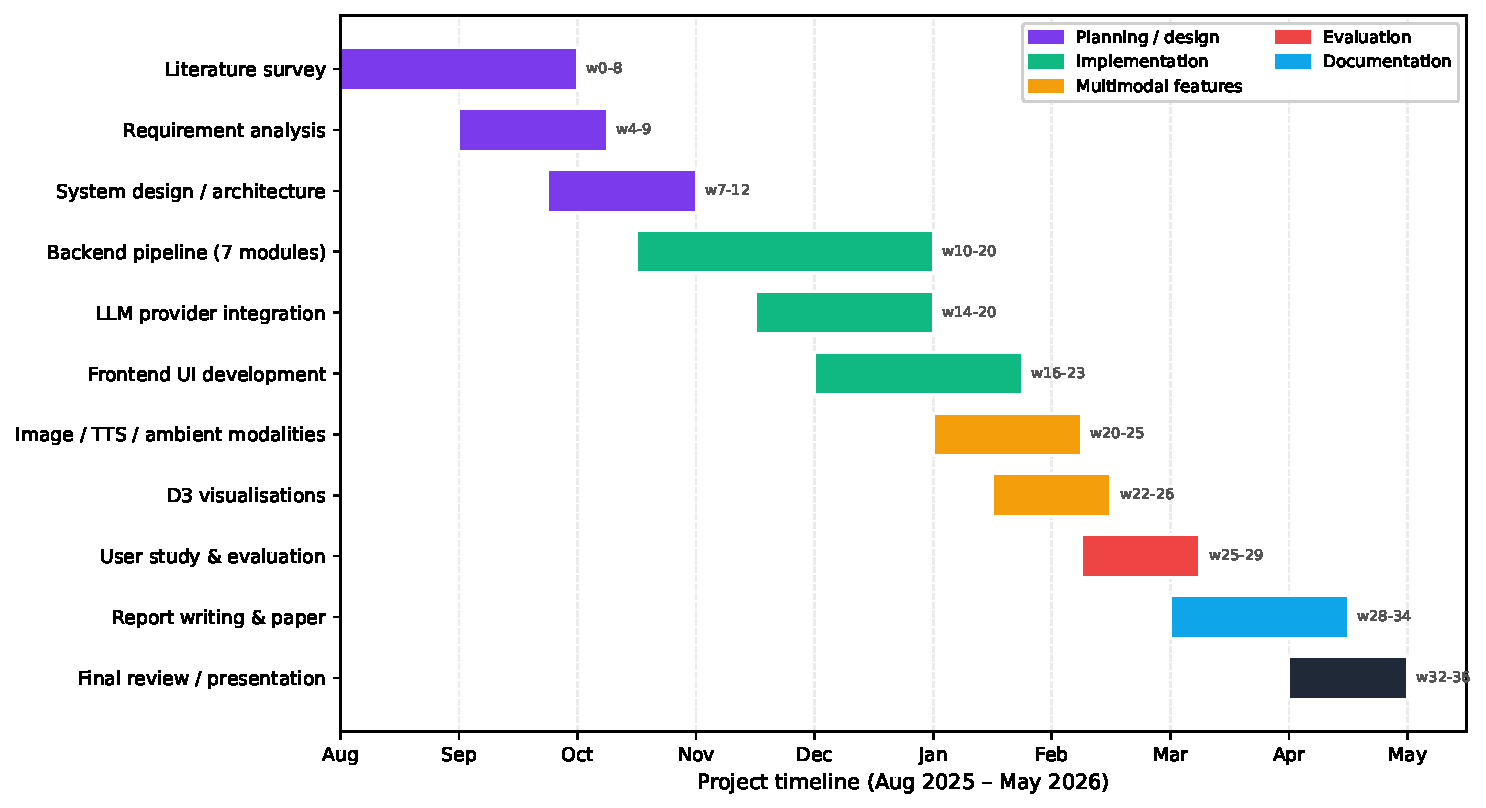
\includegraphics[width=\textwidth]{images/gantt.pdf}
    \caption{Project Gantt chart (August 2025 to May 2026).}
    \label{fig:gantt}
\end{figure}

The main risks identified during planning and the way each was handled are listed in Table~\ref{tab:risks}.

\begin{table}[H]
\centering
\caption{Risk register and mitigation.}
\label{tab:risks}
\renewcommand{\arraystretch}{1.2}
\small
\begin{tabular}{|p{4.0cm}|p{3.2cm}|p{6.0cm}|}
\hline
\textbf{Risk} & \textbf{Likelihood / Impact} & \textbf{Mitigation} \\
\hline
Rate limits of the free image API & High / High     & Serial request queue with 1.2\,s spacing and a 35\,s watchdog \\
LLM provider downtime             & Medium / Medium & Provider-independent layer that can be switched through \texttt{/api/settings} \\
Loss of narrative coherence       & Medium / High   & Sliding-window context and a consistency checker \\
Browser blocks audio autoplay     & High / Low      & Start audio only after a real user click \\
Delay in the user study           & Medium / Medium & Rolling sessions over two weeks, remote participation allowed \\
Cross-origin errors for CDN audio & Medium / Low    & Plain \texttt{HTMLAudio} without the \texttt{crossOrigin} attribute \\
\hline
\end{tabular}
\end{table}

\section{System Overview}

The system is organised in layers, shown in Figure~\ref{fig:arch}. The \emph{presentation layer} is a single-page web application that shows the questions, the story, the images and the analytics, and plays narration and music. The \emph{application layer} is a FastAPI server that exposes the REST endpoints and manages sessions. The \emph{modular core} contains the seven backend modules that turn answers into a story. At the bottom, a pluggable \emph{LLM provider layer} connects the core to Ollama, Groq, Hugging Face or OpenAI. Each layer depends only on the layer below it, so a provider can be changed or a module improved without touching the rest.

\begin{figure}[H]
    \centering
    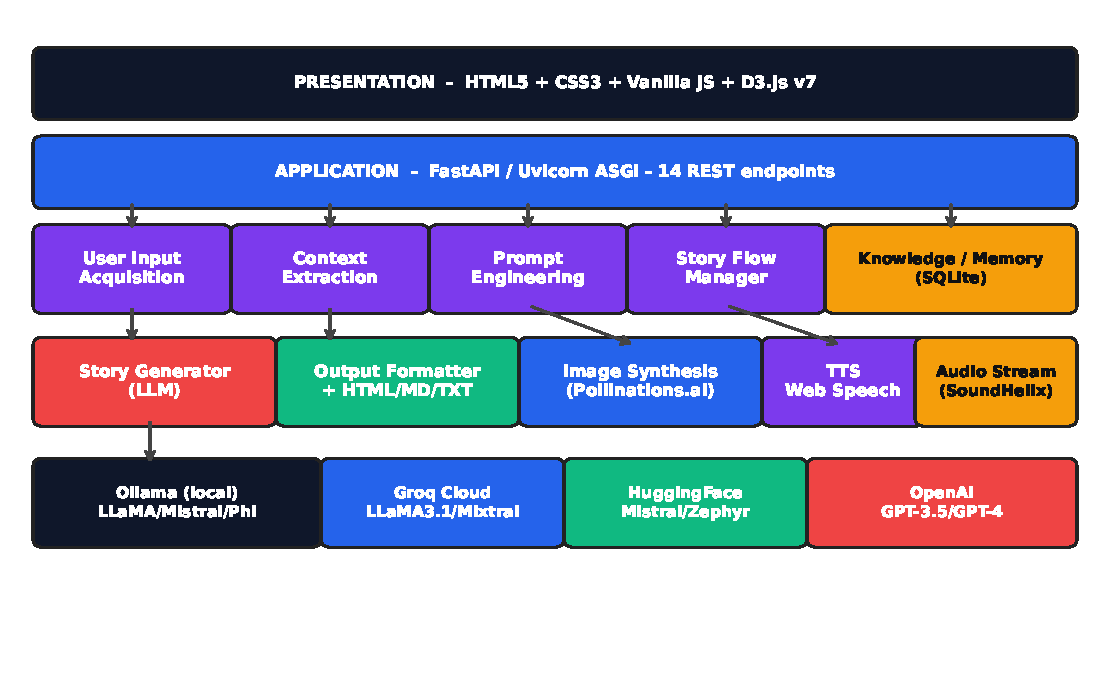
\includegraphics[width=\textwidth]{images/f07_arch.pdf}
    \caption{Layered architecture of the proposed system.}
    \label{fig:arch}
\end{figure}

\section{Research Design}

The research followed the workflow shown in Figure~\ref{fig:workflow}. Requirements were gathered from the literature and from discussion with the guide, the system was designed and built module by module, and the multimodal features were added on top of a working text pipeline. The complete system was then tested and evaluated with automatic measurements and a user study. Problems found in testing were fixed and the affected tests were run again.

\begin{figure}[H]
\centering
\begin{tikzpicture}[
    node distance=5mm,
    box/.style={draw, thick, rounded corners, fill=blue!8, minimum width=7cm, minimum height=8mm, align=center, font=\small},
    term/.style={draw, thick, ellipse, fill=green!15, minimum width=3cm, font=\small\bfseries},
    dec/.style={draw, thick, diamond, aspect=2.6, fill=orange!15, font=\small, inner sep=1pt, align=center},
    arr/.style={-{Stealth[length=2mm]}, thick}
]
\node[term] (start) {Start};
\node[box, below=of start] (a) {Literature survey and requirement analysis};
\node[box, below=of a] (b) {Design architecture, modules, API and schema};
\node[box, below=of b] (c) {Implement Q\&A, context, prompt and LLM modules};
\node[box, below=of c] (d) {Add story-flow manager and consistency checker};
\node[box, below=of d] (e) {Add images, narration, music and analytics};
\node[box, below=of e] (f) {Unit, integration, API and UI testing};
\node[dec, below=of f] (g) {All tests\\pass?};
\node[box, below=8mm of g] (h) {Evaluate: 50 stories and user study ($n=15$)};
\node[box, below=of h] (i) {Analyse results and write report};
\node[term, below=of i] (stop) {End};
\draw[arr] (start) -- (a);
\foreach \x/\y in {a/b, b/c, c/d, d/e, e/f, f/g, h/i, i/stop} \draw[arr] (\x) -- (\y);
\draw[arr] (g) -- node[right, font=\footnotesize] {Yes} (h);
\draw[arr] (g.east) -- ++(1.9,0) |- node[pos=0.25, right, font=\footnotesize] {No (fix)} (c.east);
\end{tikzpicture}
\caption{Research workflow followed in this dissertation.}
\label{fig:workflow}
\end{figure}

\section{Question-and-Answer Framework}
\label{sec:qa}

\subsection{Question Pool}

The elicitation protocol has seventeen questions divided among four narrative phases, as shown in Figure~\ref{fig:qa}:

\begin{itemize}
    \item \textbf{Setting}: the kind of world, the time period and the atmosphere of the story.
    \item \textbf{Character}: the protagonist's name, personality and goal, the antagonist, and supporting characters.
    \item \textbf{Theme}: the genre, the tone and the central message.
    \item \textbf{Plot}: the type of conflict, the plot style, the pacing and the kind of ending.
\end{itemize}

\begin{figure}[H]
    \centering
    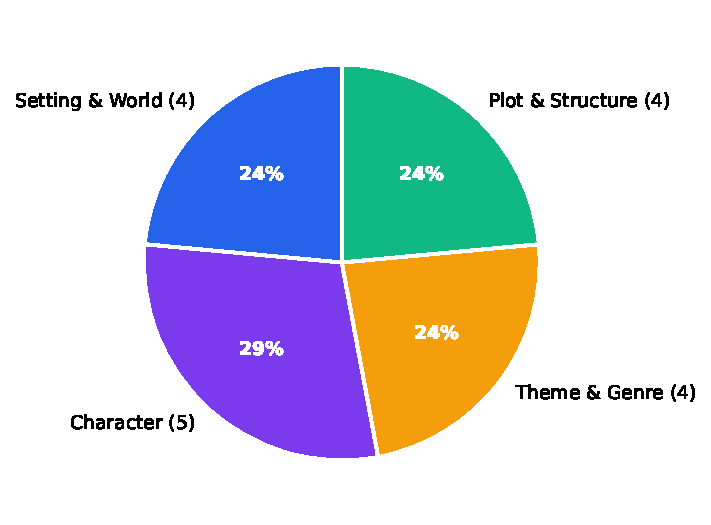
\includegraphics[width=0.65\textwidth]{images/f08_qa.pdf}
    \caption{Distribution of the 17 questions across the four phases.}
    \label{fig:qa}
\end{figure}

The user selects a budget of 4 (Quick), 8 (Balanced), 12 (Detailed) or 17 (Full) questions. The system always presents the first $N$ questions in phase order, so even the smallest budget touches all four dimensions. Every question offers multiple-choice options and a ``Write my own'' option for a free-text answer. In addition, the user may add entirely new questions with their own answers.

\subsection{Elicitation Protocol}

Let $\mathcal{Q}=\{q_1,\ldots,q_{17}\}$ be the ordered question pool. The user selects a budget $N\in\{4,8,12,17\}$ and gives an answer $a_i$ to each question $q_i$ with $i \le N$. The user may also add $M$ new question-answer pairs $(\tilde q_j, \tilde a_j)$, which receive the identifiers $\mathrm{custom\_q\_}j$. The complete response set is
\begin{equation}
R = \{(q_i, a_i)\}_{i=1}^{N} \;\cup\; \{(\mathrm{custom\_q\_}j,\ \tilde a_j)\}_{j=1}^{M},
\end{equation}
and it is sent to the context-extraction module as a JSON dictionary.

\subsection{Context Projection and Prompt Construction}

For each pair $(q_i,a_i)$ the context-extraction module applies a fixed projection $\pi_i$ that writes the answer into a typed field of a \texttt{StoryContext} object, for example \texttt{setting\_type}, \texttt{antagonist} or \texttt{plot\_style}. Answers whose identifiers are not known to the system, including all user-added questions, are stored word for word in a dictionary $D$ called \texttt{custom\_elements}. The final prompt $P$ is built as
\begin{equation}
P = T(\mathbf{c}) \oplus \sigma(D),
\end{equation}
where $T$ is the prompt template for the current story phase, $\mathbf{c}$ is the structured context, $\sigma$ turns the dictionary $D$ into a list of natural-language bullet points, and $\oplus$ joins the two strings. This design means that a new question added by the user reaches the model without any change to code or to the database schema. Figure~\ref{fig:customq} shows this routing.

\begin{figure}[H]
    \centering
    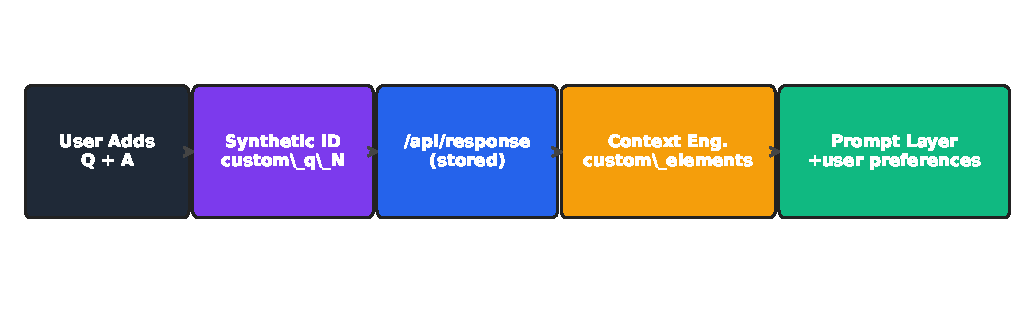
\includegraphics[width=0.95\textwidth]{images/f16_customq.pdf}
    \caption{Routing of user-added questions from the interface to the LLM prompt.}
    \label{fig:customq}
\end{figure}

\section{Five-Phase Story Progression}
\label{sec:phases}

The story-flow manager is a finite-state machine based on Freytag's pyramid~\citep{freytag1900drama}. The story moves through five phases according to its total word count, as listed in Table~\ref{tab:phases}. The current phase selects the prompt template: the introduction template asks the model to set the scene and introduce the characters, the climax template asks for the main confrontation, and the resolution template asks the model to close open plot threads. Figure~\ref{fig:phases} shows the observed word counts per phase; the rising action takes the largest share of the text (about 820 words), which agrees with narrative theory.

\begin{table}[H]
\centering
\caption{Word-count thresholds of the five story phases.}
\label{tab:phases}
\renewcommand{\arraystretch}{1.2}
\begin{tabular}{|l|c|l|}
\hline
\textbf{Phase} & \textbf{Word range} & \textbf{Purpose of the prompt} \\
\hline
Introduction   & 0--400       & Establish setting and characters \\
Rising action  & 400--1200    & Develop conflict and complications \\
Climax         & 1200--1800   & Main confrontation or turning point \\
Falling action & 1800--2400   & Consequences of the climax \\
Resolution     & $>$ 2400     & Resolve open threads and conclude \\
\hline
\end{tabular}
\end{table}

\begin{figure}[H]
    \centering
    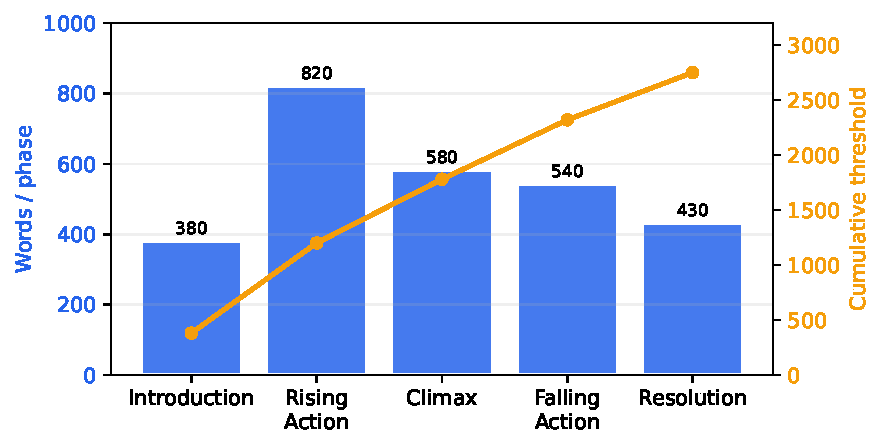
\includegraphics[width=0.9\textwidth]{images/f04_phases.pdf}
    \caption{Word-count distribution across the five story phases.}
    \label{fig:phases}
\end{figure}

\section{Generation Loop}

Each turn of the story follows Algorithm~\ref{alg:loop}. The model sees the structured context and only the last $k$ segments of the story, which keeps the prompt within the context window while preserving the most recent events. Image generation starts in parallel with post-processing so that the picture is often ready when the user finishes reading.

\begin{algorithm}[H]
\caption{Story generation loop for one turn}
\label{alg:loop}
\begin{algorithmic}[1]
\Require session $s$, structured context $\mathbf{c}$, custom elements $D$, user choice $u$ (empty on the first turn)
\Ensure formatted segment and choices for the next turn
\State $H \gets$ last $k$ segments of session $s$ \Comment{sliding window, $k=4$}
\State $\phi \gets$ current phase from total word count
\State $P \gets T_{\phi}(\mathbf{c}, H, u) \oplus \sigma(D)$
\State $y \gets \textsc{LLM}(P)$ \Comment{active provider}
\State $y \gets \textsc{Format}(y)$ \Comment{clean text, style dialogue}
\State update character and plot-thread trackers with $y$
\State run consistency checks on $y$ against $H$ and $\mathbf{c}$
\State start image request for $y$ asynchronously
\State save $y$ to the database; update word count
\State \Return $y$ and generated choices
\end{algorithmic}
\end{algorithm}

\section{Backend Modules}
\label{sec:modules}

The backend has seven modules with clear responsibilities and typed Pydantic interfaces.

\subsection{Module 1: User Input Acquisition}

This module holds the question pool and serves it through two endpoints: \texttt{/api/questions/all} returns all questions grouped by phase, and \texttt{/api/question/next} supports an older one-question-at-a-time mode. Answers are received through \texttt{POST /api/response} and validated. The landing page (Figure~\ref{fig:ui-landing}) lets the user choose a budget, and the question form (Figure~\ref{fig:ui-form}) shows each question with its options and a dashed ``Write my own'' chip.

\begin{figure}[H]
    \centering
    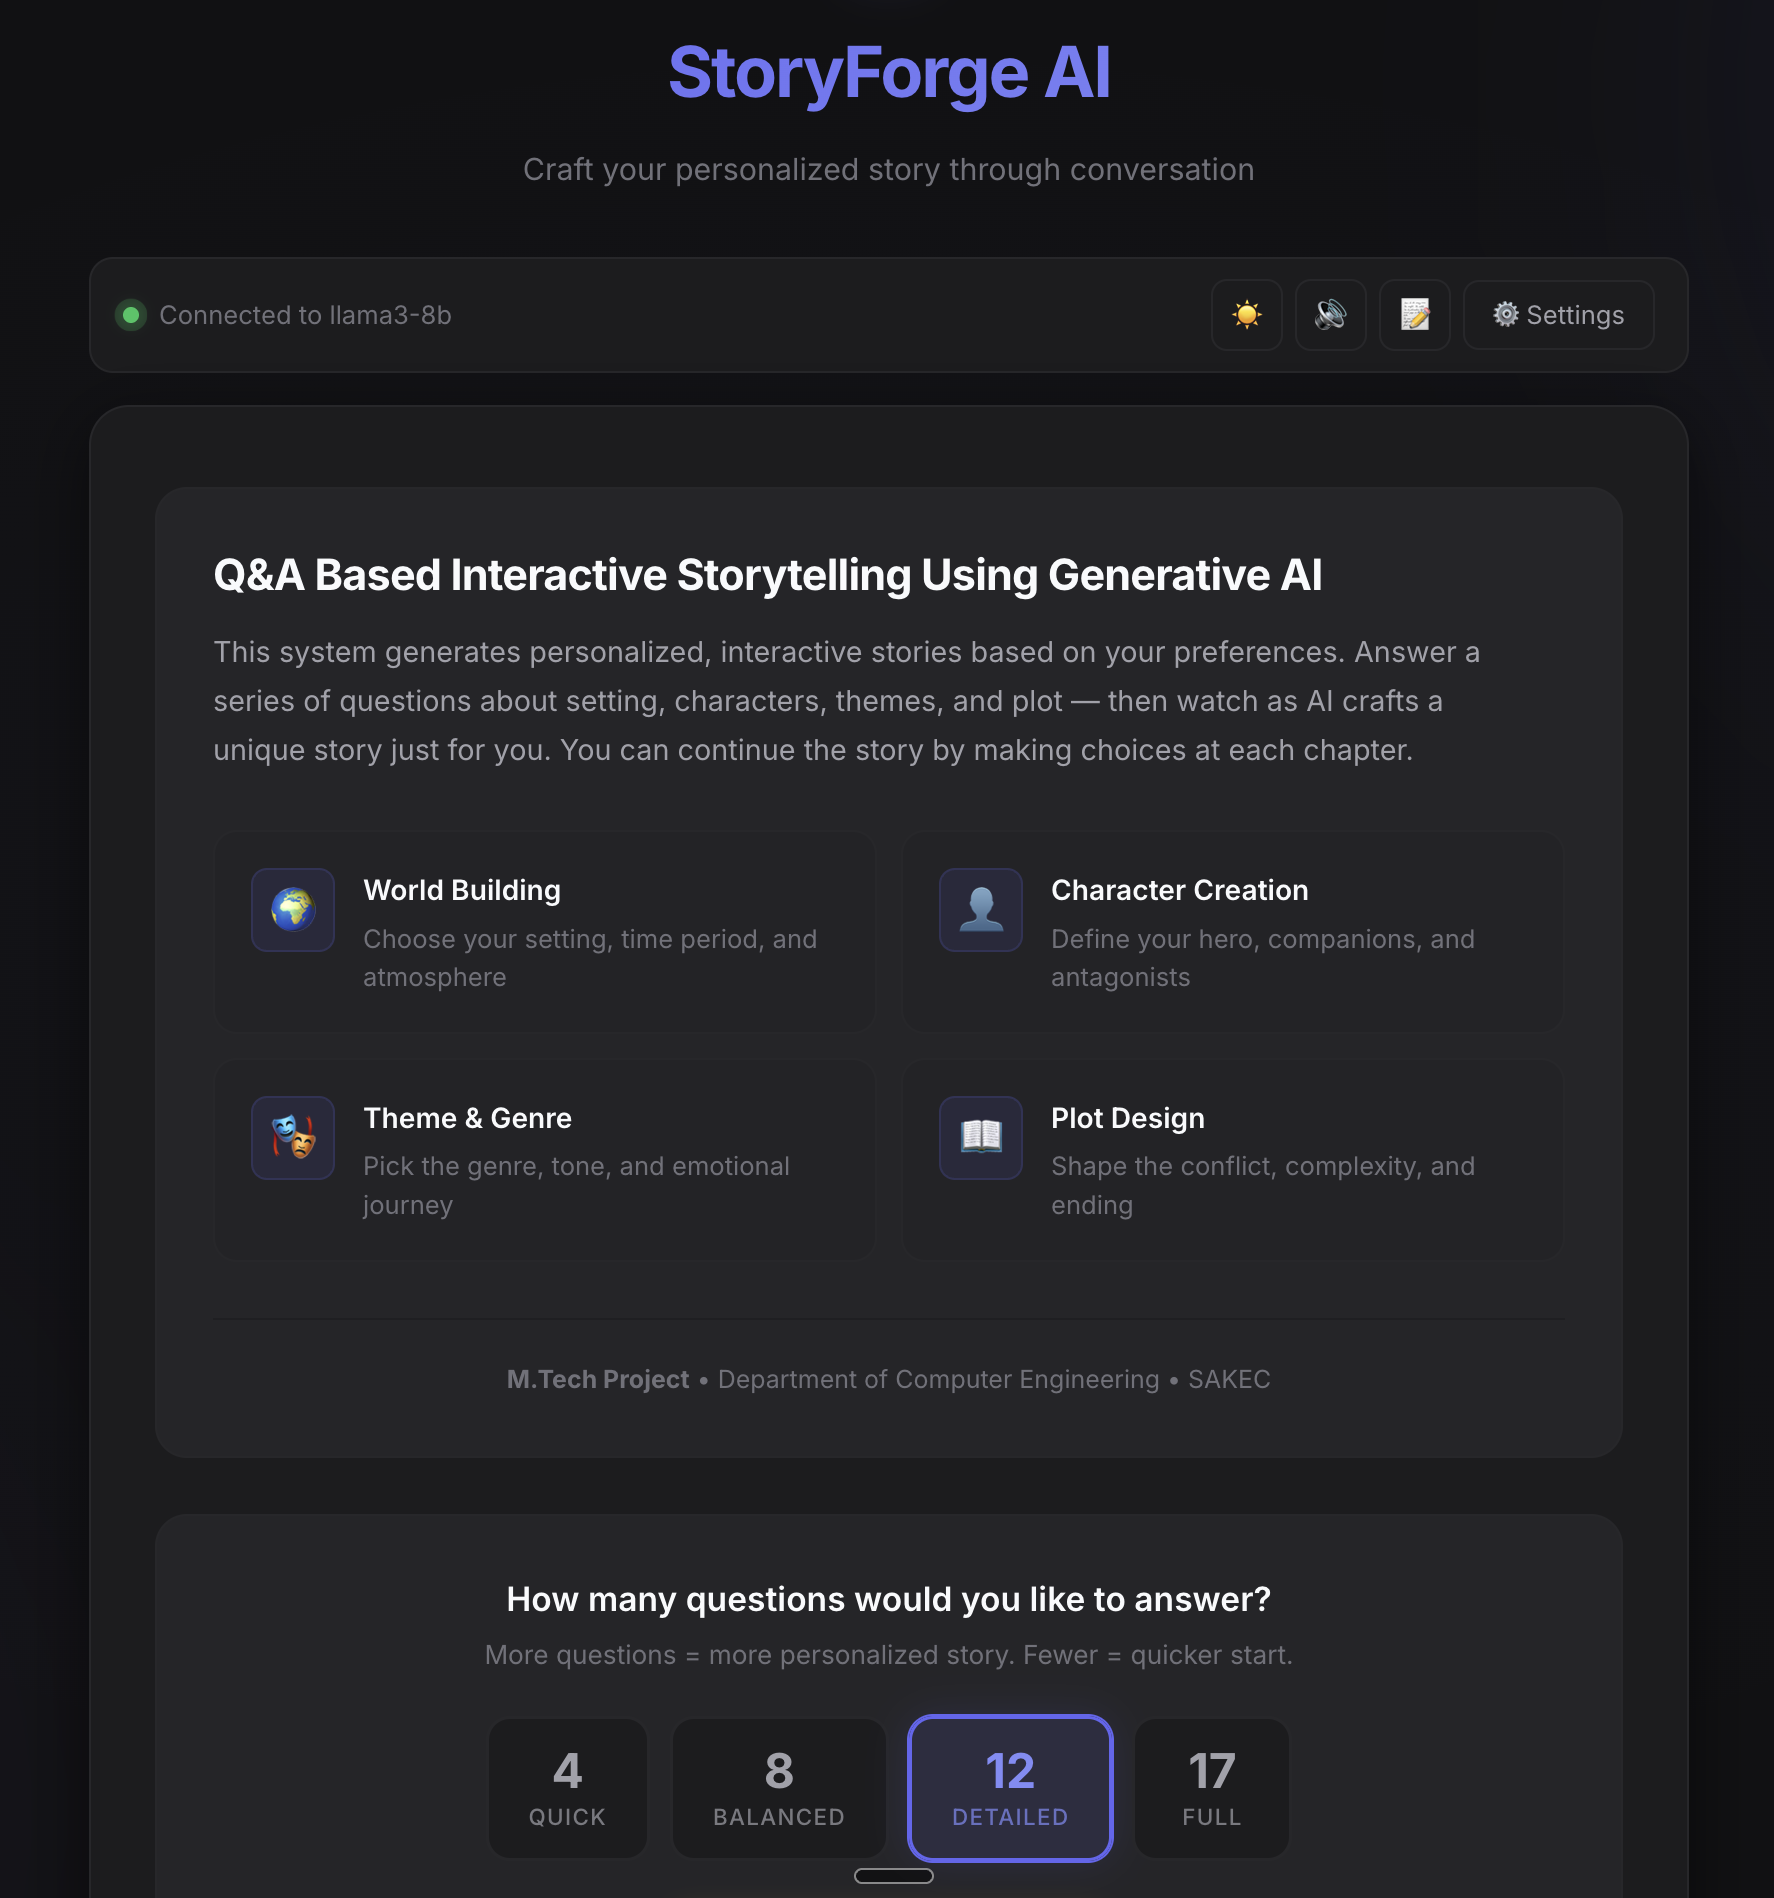
\includegraphics[width=0.85\textwidth]{images/s01_landing.png}
    \caption{Landing page with the choice of question budget.}
    \label{fig:ui-landing}
\end{figure}

\begin{figure}[H]
    \centering
    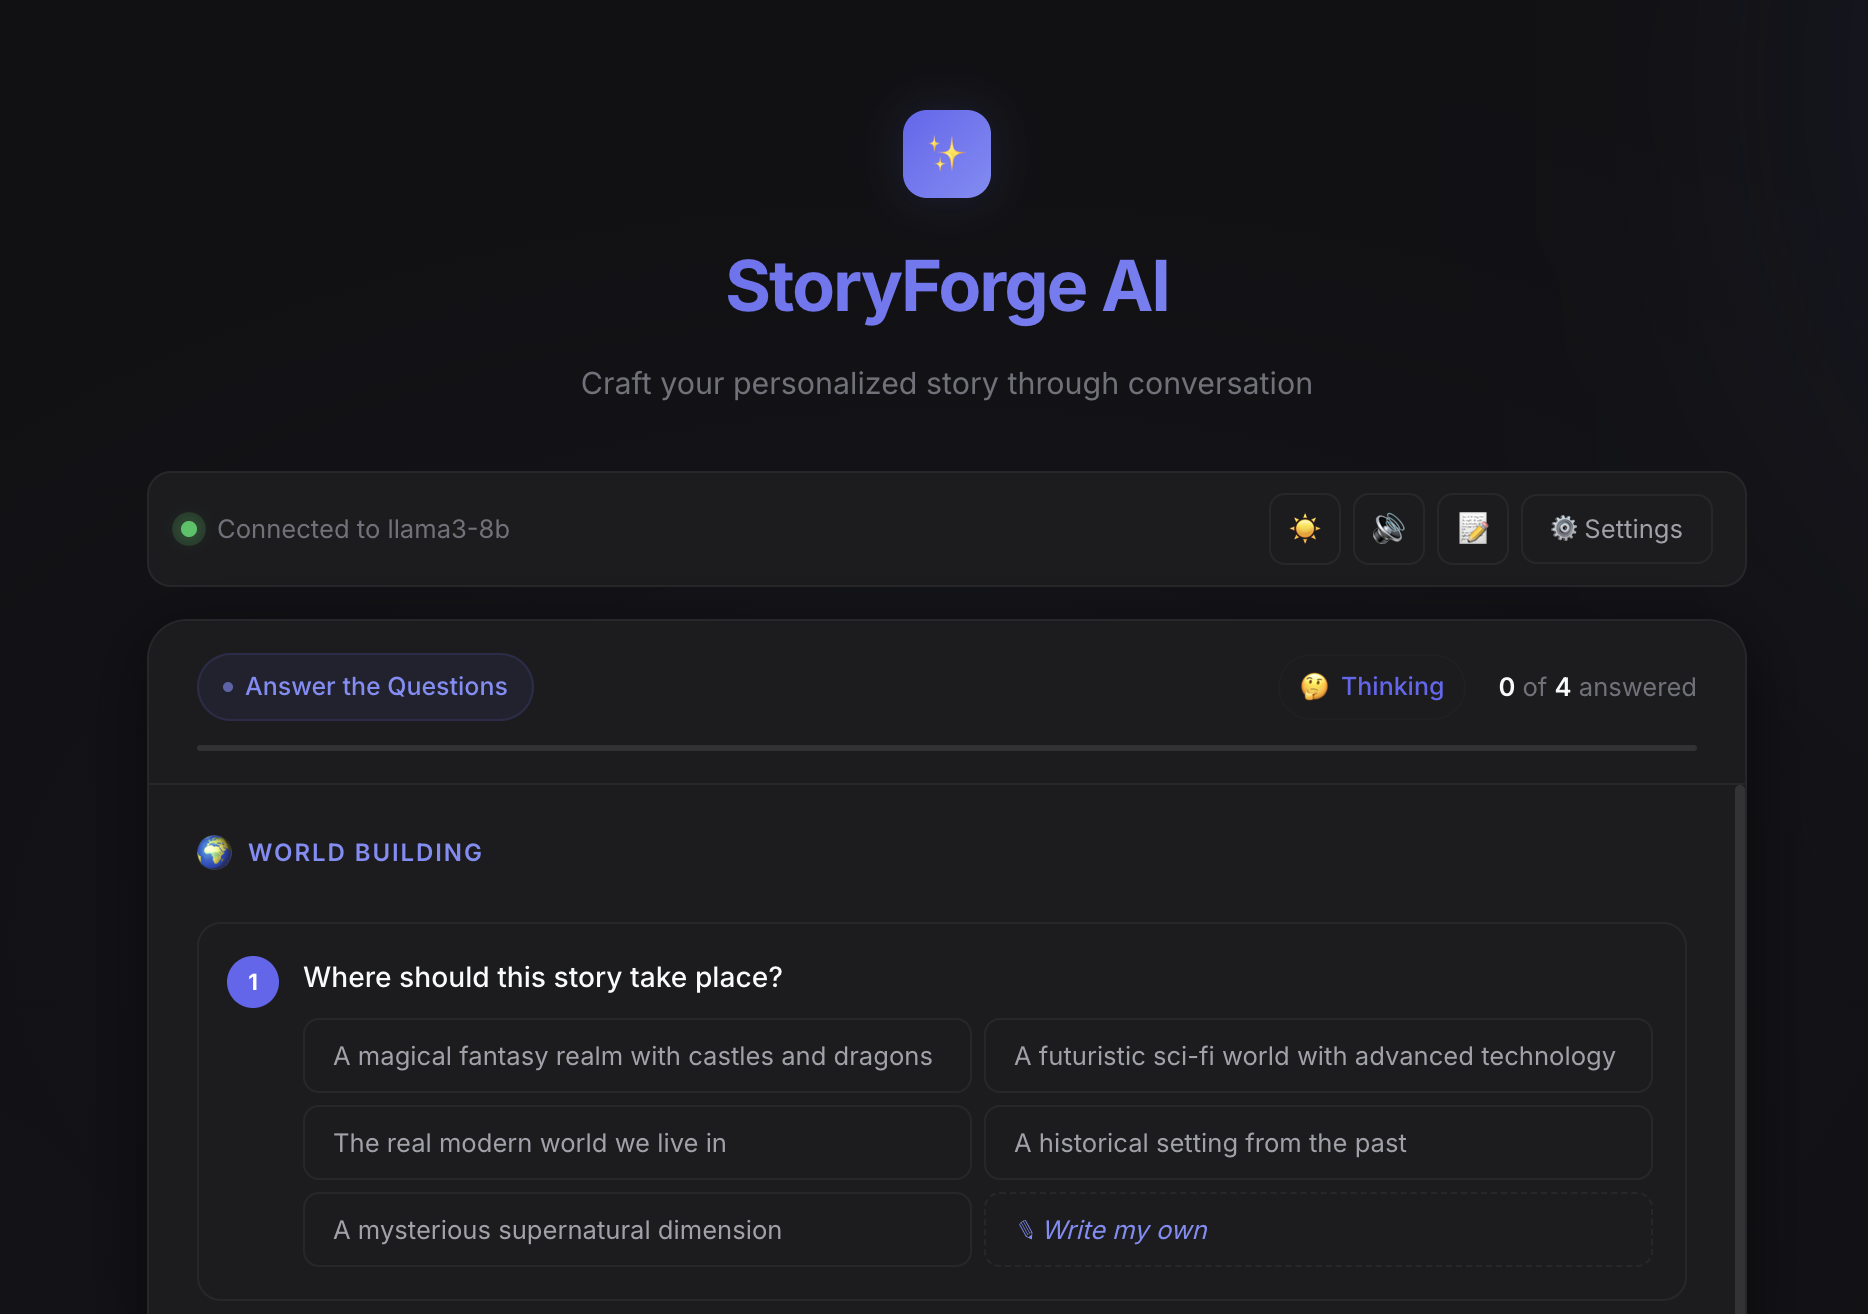
\includegraphics[width=0.85\textwidth]{images/s02_questions.png}
    \caption{Single-page question form with custom-answer option.}
    \label{fig:ui-form}
\end{figure}

\subsection{Module 2: Context Extraction Engine}

This module fills the \texttt{StoryContext} object. It works in two passes: first it classifies answers with keyword dictionaries (six genres, five setting types and five conflict types), and then it extracts proper names with regular expressions. Identifiers that begin with \texttt{custom\_} are routed into \texttt{custom\_elements}:

\begin{lstlisting}[language=Python]
elif question_id.startswith("custom_"):
    self.context.custom_elements[question_id] = answer
\end{lstlisting}

\subsection{Module 3: Knowledge and Memory}

This module stores sessions, answers, segments and preferences in SQLite, keeps an in-memory LRU cache for active sessions, and provides the sliding-window helper used in Algorithm~\ref{alg:loop}:

\begin{lstlisting}[language=Python]
def get_recent_context(session_id: str, k: int = 4) -> str:
    """Return the concatenated text of the last k segments."""
\end{lstlisting}

\subsection{Module 4: Prompt Engineering}

This module holds six prompt families: the system prompt, the initial-segment prompt, the continuation prompt, the climax prompt, the resolution prompt and the choice-generation prompt. Each is filled with fields from \texttt{StoryContext}, and genre-specific guidance is added (for example, magic systems for fantasy, clue placement and red herrings for mystery, and emotional pacing for romance). User-added preferences are appended at the end:

\begin{lstlisting}[language=Python]
if context.custom_elements:
    extras = "\n".join(f"- {v}" for v in context.custom_elements.values() if v)
    if extras:
        prompt += "\n\nAdditional user preferences to honour:\n" + extras
\end{lstlisting}

\subsection{Module 5: Story Generator}

The story generator defines an abstract class \texttt{BaseLLMClient} with four concrete clients, compared in Table~\ref{tab:providers}. A factory creates the client named in the configuration. The settings panel (Figure~\ref{fig:ui-settings}) lets a non-technical user choose the provider, model, temperature and features; a change is sent to \texttt{POST /api/settings}, which replaces the client without restarting the server.

\begin{table}[H]
\centering
\caption{LLM providers supported by the system.}
\label{tab:providers}
\renewcommand{\arraystretch}{1.2}
\begin{tabular}{|l|l|l|c|}
\hline
\textbf{Provider} & \textbf{Models} & \textbf{Cost} & \textbf{Latency} \\
\hline
Ollama       & LLaMA 3.2, Mistral, Phi    & Free (local)        & 8--15\,s \\
Groq         & LLaMA 3.1 8B/70B, Mixtral  & Free, 14,400/day    & 1--3\,s \\
Hugging Face & Mistral-7B, Zephyr, Falcon & Free (rate-limited) & 6--10\,s \\
OpenAI       & GPT-3.5-turbo, GPT-4       & Paid per token      & 2--4\,s \\
\hline
\end{tabular}
\end{table}

\begin{figure}[H]
    \centering
    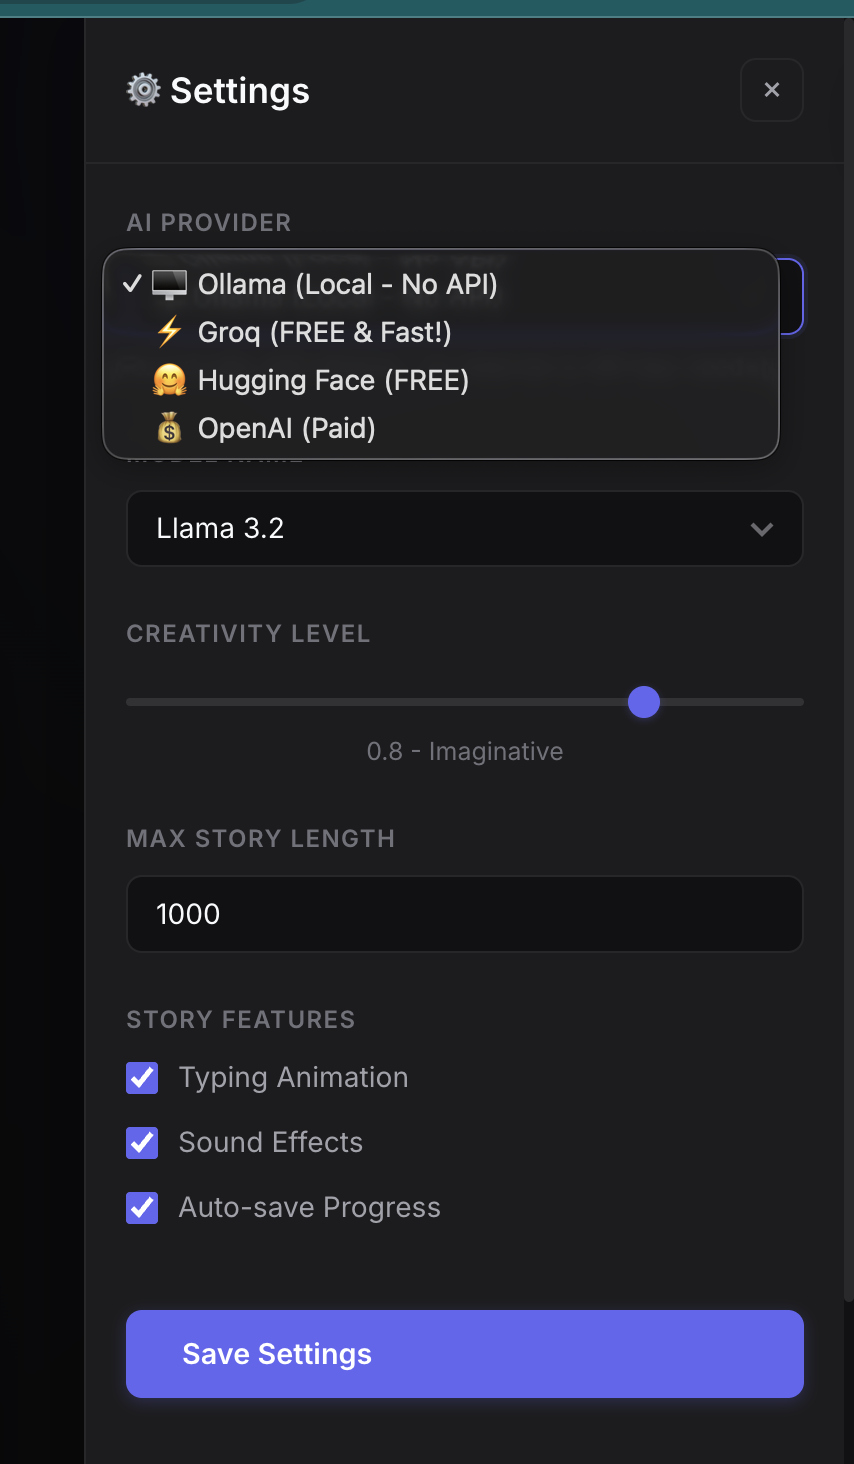
\includegraphics[width=0.55\textwidth]{images/s05_settings.png}
    \caption{Settings panel for provider, model, temperature and feature toggles.}
    \label{fig:ui-settings}
\end{figure}

\subsection{Module 6: Story Flow Manager}

This module implements the five-phase state machine of Section~\ref{sec:phases}. A \texttt{CharacterTracker} records each character's mentions and traits, and a \texttt{PlotThreadTracker} records open plot threads. The consistency checker uses both to flag five kinds of problem: character contradictions, abandoned plot threads, pacing problems, setting inconsistencies and tone shifts.

\subsection{Module 7: Output Formatter}

The formatter cleans the model's output by collapsing extra whitespace and fixing quote and dash characters, splits text at sentence boundaries, wraps dialogue in styled HTML spans, and exports the full story as plain text, Markdown or HTML.

\section{Multimodal Pipelines}

\subsection{Scene Illustration}

For each segment, a short image prompt is built from the most visual sentence. Dialogue in quotation marks and sentences built around thought verbs (\emph{thought, remembered, wondered}) are removed first, because they describe things that cannot be drawn. Each remaining sentence $s$ is scored as
\begin{equation}
\mathrm{score}(s) = 2 \cdot \mathbf{1}_{V}(s) - 2 \cdot \mathbf{1}_{T}(s) + \min\bigl(3,\ |\mathrm{ProperNouns}(s)|\bigr),
\end{equation}
where $\mathbf{1}_V(s)$ is 1 if the sentence contains a visual verb (\emph{stood, loomed, soared, glowed, towered}, and so on) and $\mathbf{1}_T(s)$ is 1 if it contains a thought verb. The best sentence is combined with the genre, the current mood and a fixed style prefix, and the prompt is limited to 200 characters. The pipeline is shown in Figure~\ref{fig:imgpipe}.

\begin{figure}[H]
    \centering
    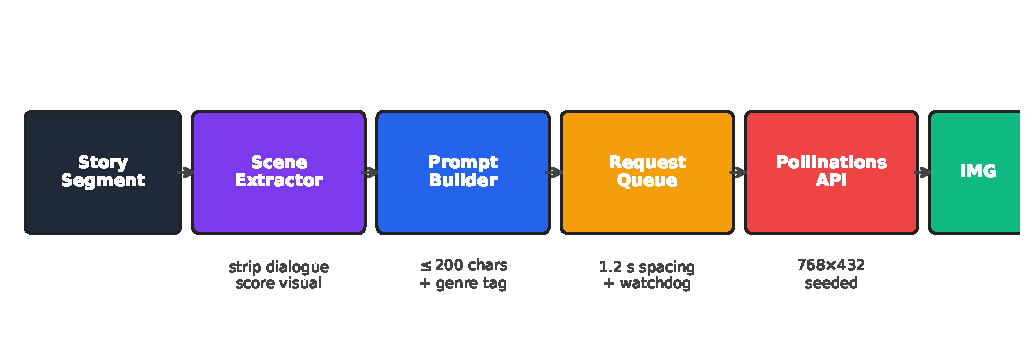
\includegraphics[width=0.95\textwidth]{images/f09_imgpipe.pdf}
    \caption{Per-segment image synthesis pipeline.}
    \label{fig:imgpipe}
\end{figure}

The prompt is sent to Pollinations.ai as a URL:

\begin{lstlisting}
imageUrlFor(segmentText, seed, opts={}) {
    const prompt = this.buildImagePrompt(segmentText, opts);
    const params = new URLSearchParams({
        width: '768', height: '432', nologo: 'true',
        seed: String(seed)
    });
    return `https://image.pollinations.ai/prompt/${encodeURIComponent(prompt)}?${params}`;
}
\end{lstlisting}

Pollinations is served through Cloudflare, which rejects bursts of parallel requests. All image requests therefore pass through a serial queue that sends one request at a time, waits 1.2\,s between requests, and abandons a request after a 35\,s watchdog so that a hung request cannot block the queue. Figure~\ref{fig:ui-loading} shows the loading state while the LLM call and the image request run, and Figure~\ref{fig:ui-story} shows a finished segment with its illustration.

\begin{figure}[H]
    \centering
    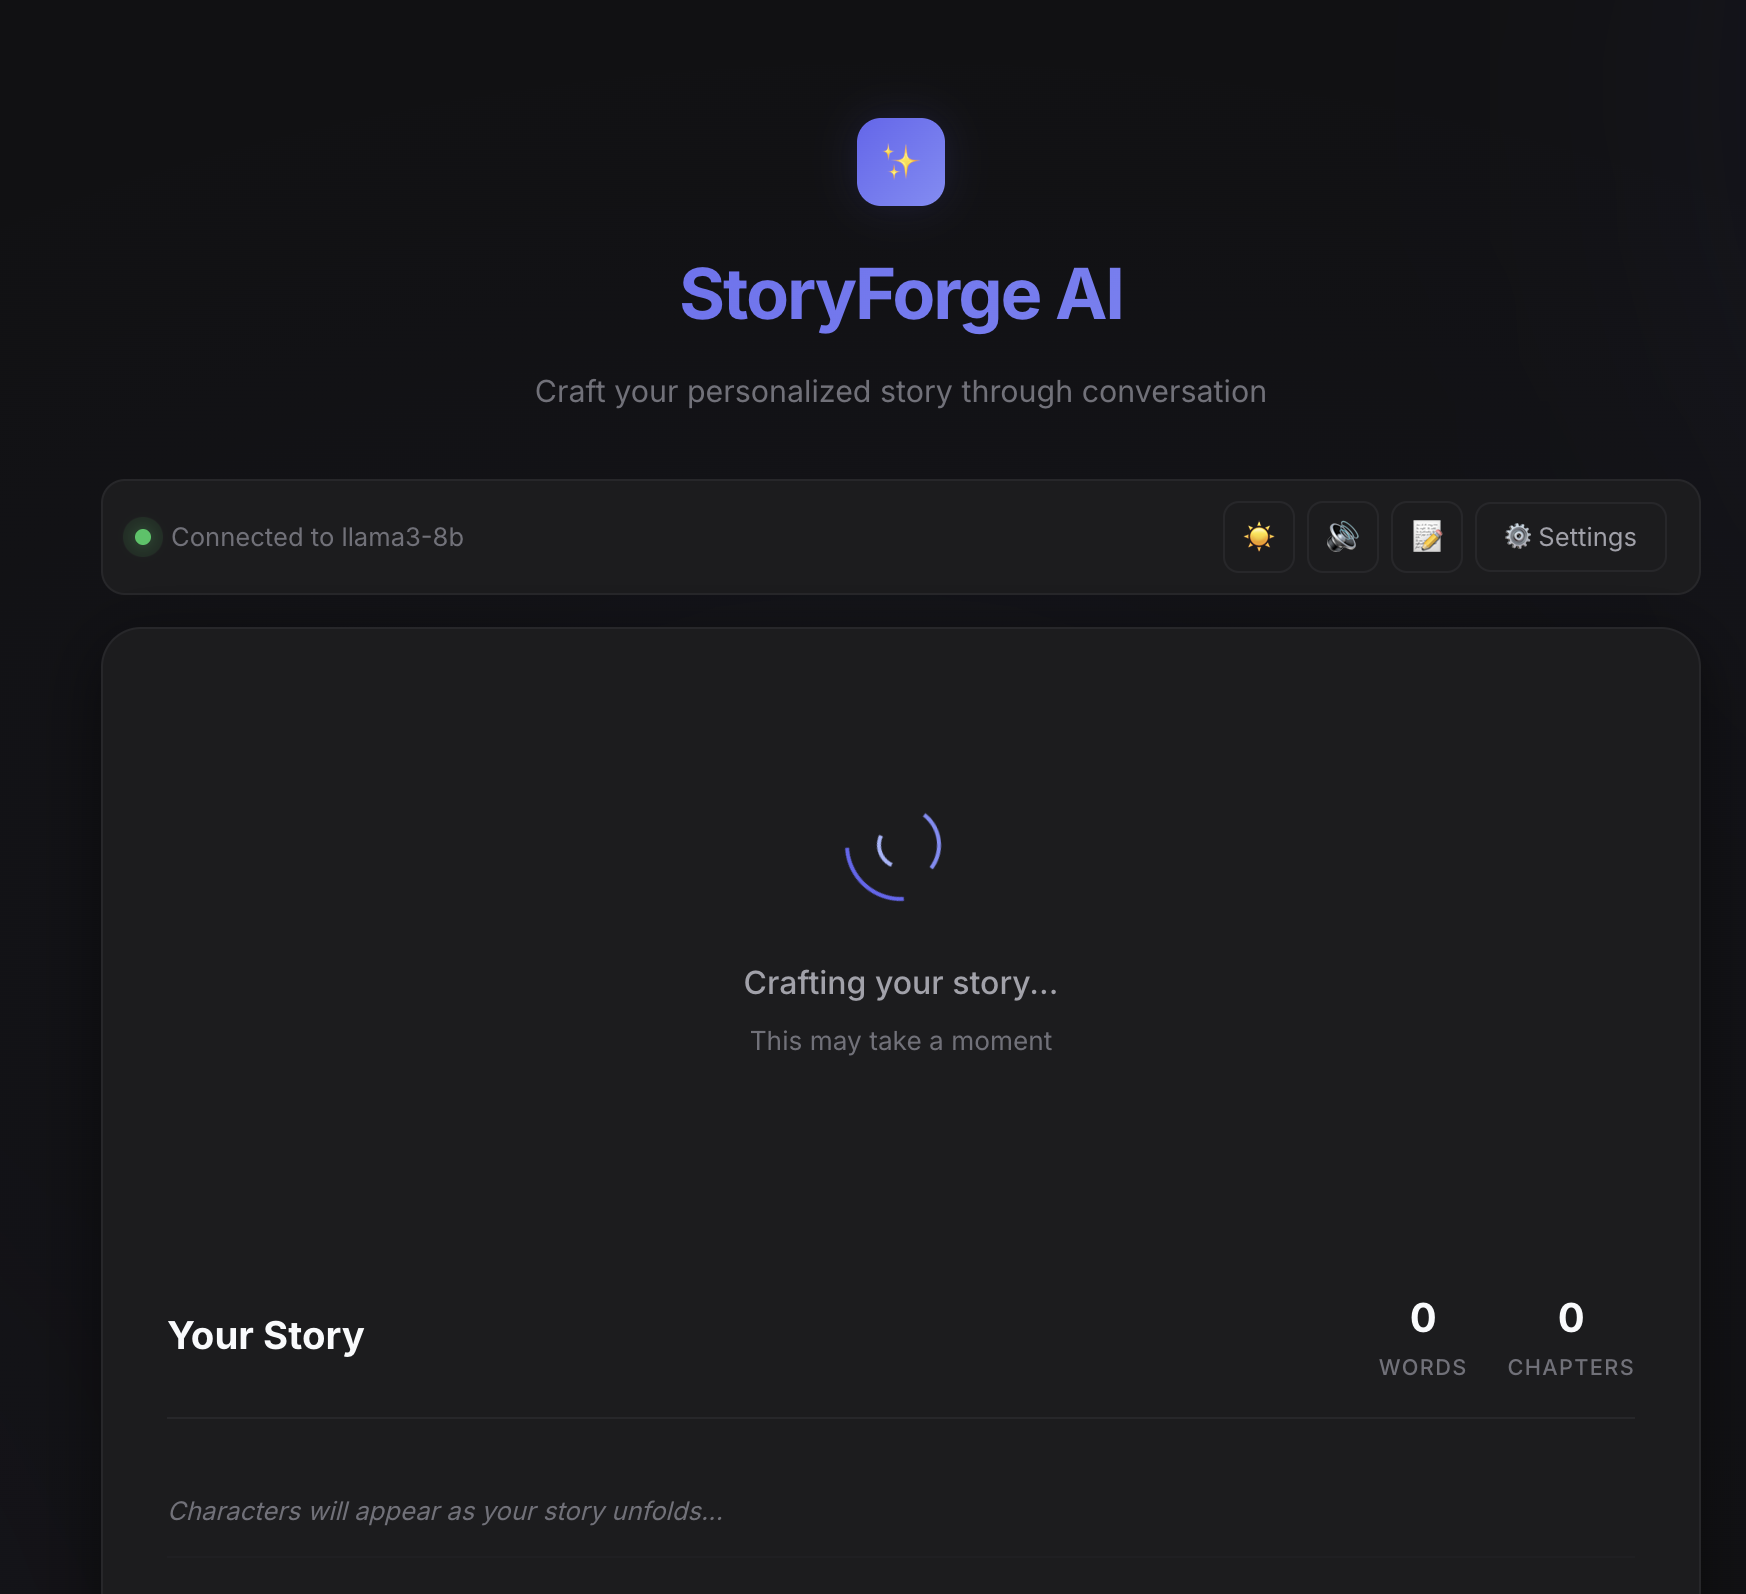
\includegraphics[width=0.85\textwidth]{images/s03_loading.png}
    \caption{Loading state during story and image generation.}
    \label{fig:ui-loading}
\end{figure}

\begin{figure}[H]
    \centering
    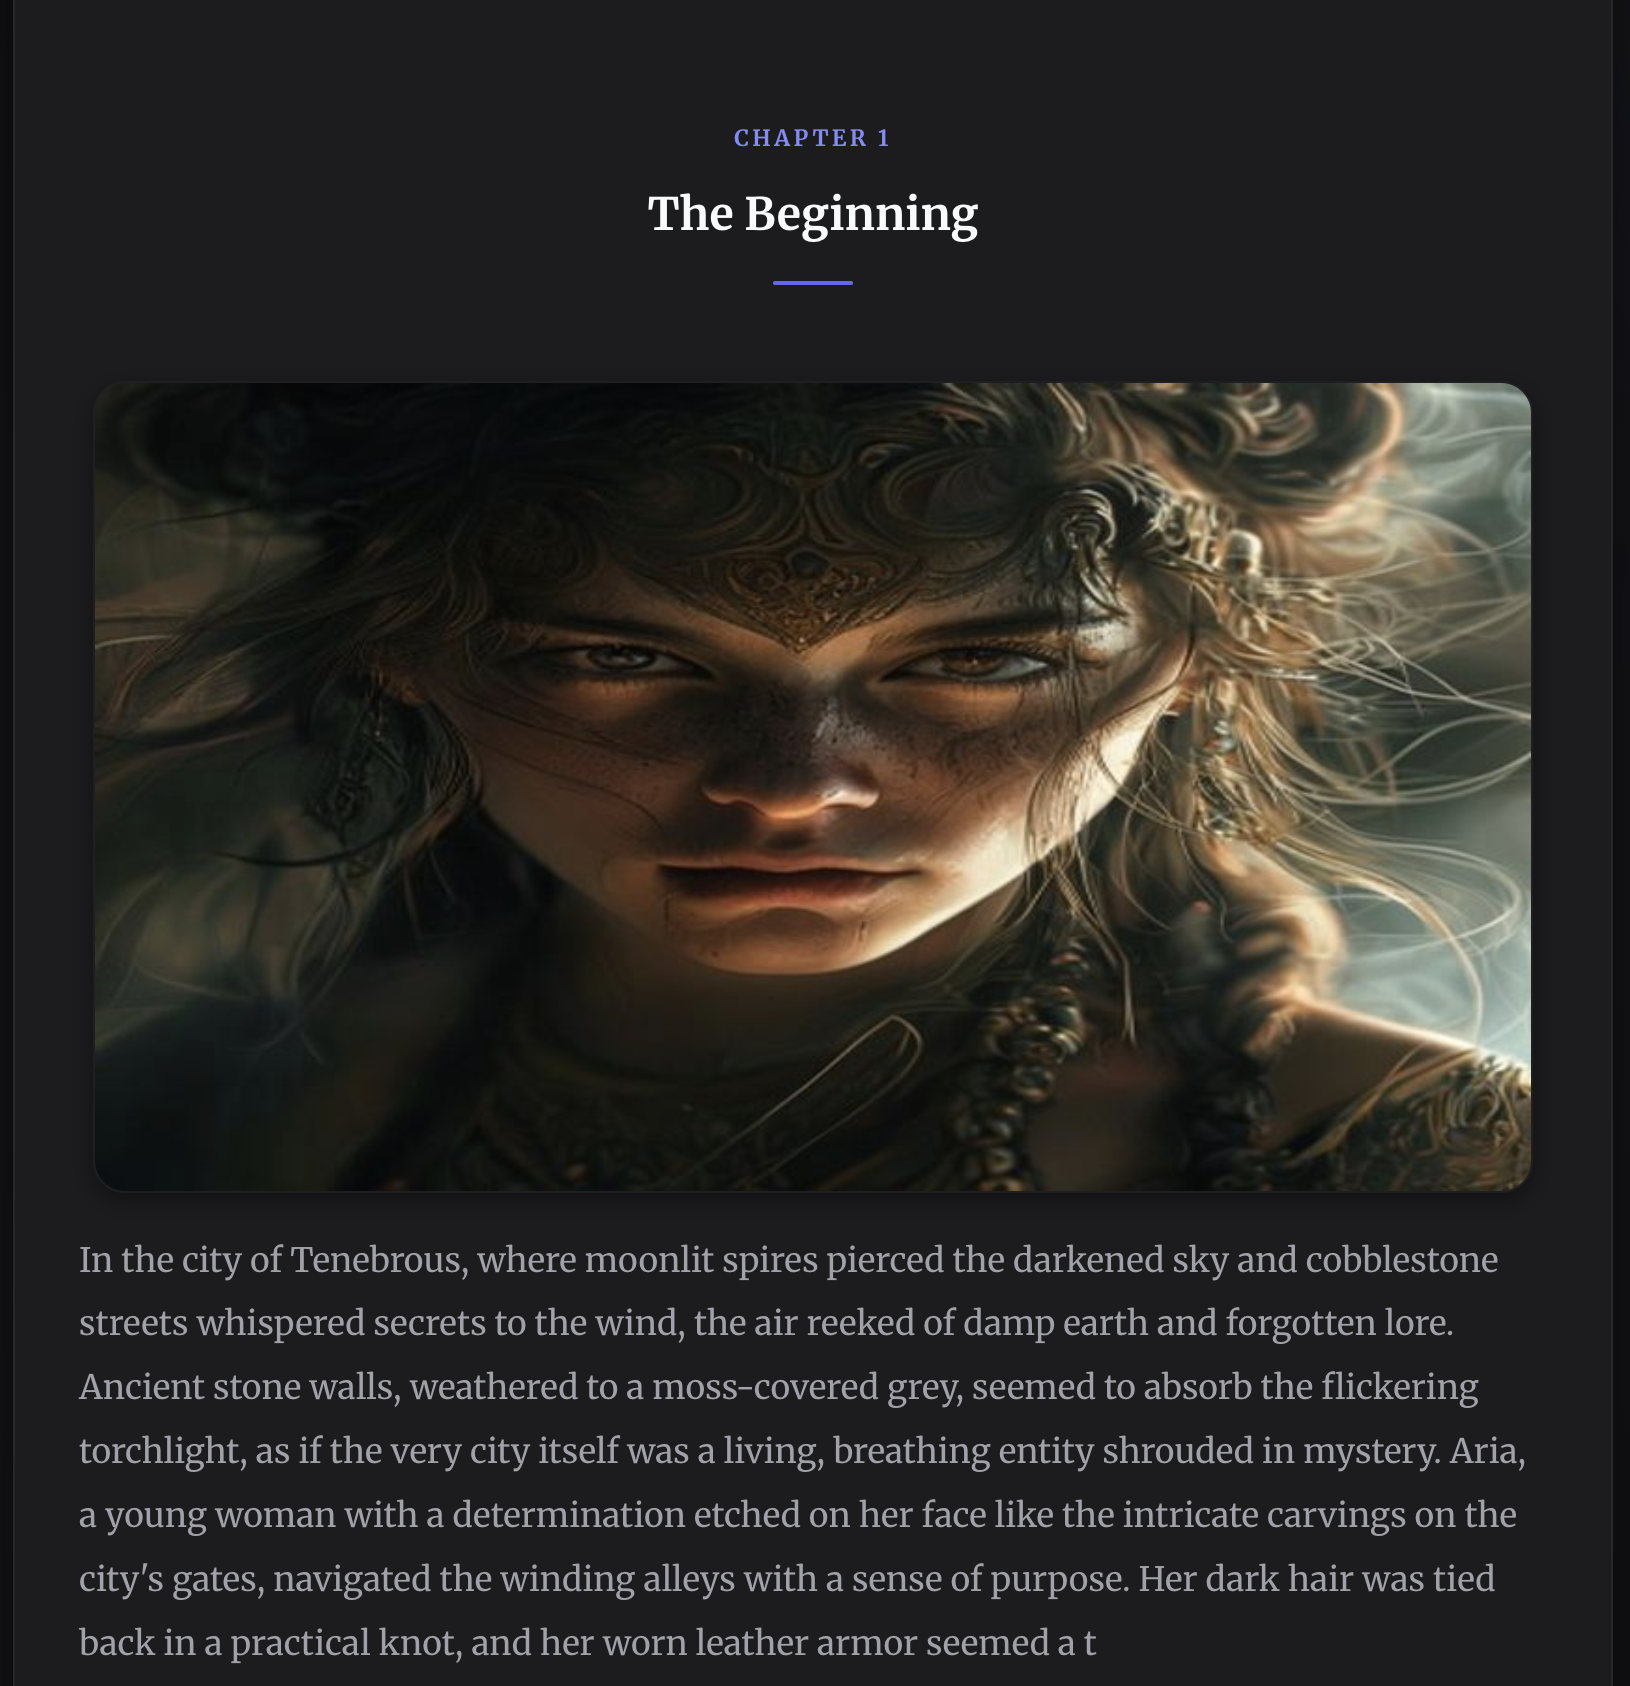
\includegraphics[width=0.65\textwidth]{images/s04_story_image.png}
    \caption{Generated story segment with its scene illustration.}
    \label{fig:ui-story}
\end{figure}

\subsection{Narration and Ambient Music}

The two audio pipelines are shown in Figure~\ref{fig:audio}. Narration uses the browser's \texttt{window.speechSynthesis} interface. One utterance is queued per segment, with pause, resume and stop controls, and the voice is the one provided by the operating system. Ambient music maps each of eight genres to a SoundHelix track, played through \texttt{HTMLAudio} in a loop with a 2.4\,s fade-in and a 0.8\,s fade-out. The \texttt{crossOrigin} attribute is not set, because the CDN does not return CORS headers; setting it caused loading to fail in an early version.

\begin{figure}[H]
    \centering
    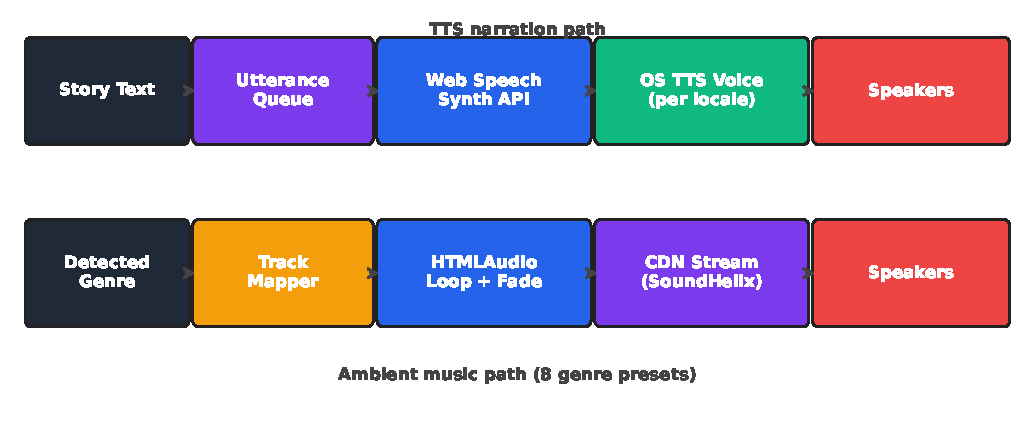
\includegraphics[width=0.95\textwidth]{images/f10_audio.pdf}
    \caption{Narration and ambient-music signal flows.}
    \label{fig:audio}
\end{figure}

\section{Reader Analytics}

\subsection{Story Map}

The Story Map arranges the chapters as a vertical tree using \texttt{d3.tree()}. Each node shows an 80-character preview of its chapter and the user choice that led to it, so the reader can see how the story branched.

\subsection{Character Relationship Graph}

Capitalised words are taken from the segment text and filtered with an extended stop-word list. Only names that appear at least twice are kept. For every pair of kept names, the edge weight is the number of segments in which both appear, and the node radius grows with the number of mentions. The graph is drawn with a D3 force layout (link distance 110, charge $-220$, collision radius 34 pixels). Because the edges are based only on co-appearance, the modal states clearly that the graph shows which characters appear together and not the type of relationship between them.

\section{System Implementation}

\subsection{Project Structure}

The source code is organised as follows and is available as open source~\citep{jha2026repo}:

\begin{lstlisting}
AI-Story-Generator/
|-- main.py                    # FastAPI entry point, REST endpoints
|-- config.py                  # provider, model, temperature
|-- requirements.txt
|-- app/
|   |-- modules/
|   |   |-- user_input.py            # 17 questions, 4 phases
|   |   |-- context_extraction.py    # StoryContext + custom_elements
|   |   |-- knowledge_memory.py      # SQLite + LRU cache
|   |   |-- prompt_engineering.py    # 6 prompt families
|   |   |-- story_generator.py       # BaseLLMClient + 4 providers
|   |   |-- story_flow_manager.py    # 5-phase FSM + trackers
|   |   `-- output_formatter.py      # TXT/MD/HTML export
|   |-- templates/index.html         # single-page shell
|   `-- static/css/style.css, js/app.js
`-- data/storytelling.db
\end{lstlisting}

\subsection{Database Schema}

The SQLite database has five tables:

\begin{lstlisting}
sessions         (session_id PK, user_id, created_at, status)
story_segments   (id PK, session_id FK, order, content, user_choice)
story_context    (session_id PK/FK, context_json, updated_at)
qa_history       (id PK, session_id FK, question_id, q_text, a_text)
user_preferences (user_id PK, preferences_json, updated_at)
\end{lstlisting}

\subsection{REST API}

The server exposes the endpoints listed in Table~\ref{tab:rest}. All request and response bodies are typed with Pydantic~v2.

\begin{table}[H]
\centering
\caption{REST API endpoints.}
\label{tab:rest}
\renewcommand{\arraystretch}{1.2}
\small
\begin{tabular}{|l|c|l|}
\hline
\textbf{Endpoint} & \textbf{Method} & \textbf{Purpose} \\
\hline
\texttt{/}                           & GET    & Web interface \\
\texttt{/api/status}                 & GET    & Check LLM availability \\
\texttt{/api/session/new}            & POST   & Create a new session \\
\texttt{/api/questions/all}          & GET    & All questions, grouped by phase \\
\texttt{/api/question/next}          & GET    & Next question (sequential mode) \\
\texttt{/api/response}               & POST   & Submit an answer \\
\texttt{/api/story/generate}         & POST   & Generate the first segment \\
\texttt{/api/story/continue}         & POST   & Continue from a user choice \\
\texttt{/api/story/full/\{id\}}      & GET    & Full story of a session \\
\texttt{/api/story/download/\{id\}}  & GET    & Export as TXT, MD or HTML \\
\texttt{/api/settings}               & POST   & Switch provider or model \\
\texttt{/api/session/\{id\}/summary} & GET    & Session statistics \\
\texttt{/api/session/\{id\}}         & DELETE & End a session \\
\hline
\end{tabular}
\end{table}

\subsection{Technology Stack}

The software used is listed in Table~\ref{tab:stack}. All components are free, and most are open source.

\begin{table}[H]
\centering
\caption{Technology stack.}
\label{tab:stack}
\renewcommand{\arraystretch}{1.2}
\small
\begin{tabular}{|l|l|l|}
\hline
\textbf{Layer} & \textbf{Technology} & \textbf{Purpose} \\
\hline
Operating system & macOS 14 / Ubuntu 22.04          & Development host \\
Backend language & Python 3.9+                      & Core logic \\
Web framework    & FastAPI with Uvicorn             & REST API and templates \\
Frontend         & HTML5, CSS3, JavaScript          & Single-page interface \\
Visualisation    & D3.js v7                         & Story Map, Character Graph \\
Database         & SQLite3 with aiosqlite           & Sessions, answers, segments \\
HTTP client      & httpx (async)                    & Calls to LLM providers \\
Schemas          & Pydantic v2                      & Request and response types \\
Image service    & Pollinations.ai                  & Text-to-image \\
Speech           & W3C Web Speech Synthesis API     & Narration \\
Ambient audio    & HTMLAudio with SoundHelix        & Genre music \\
LLM providers    & Ollama, Groq, Hugging Face, OpenAI & Story generation \\
\hline
\end{tabular}
\end{table}

\subsection{Hardware Requirements}

Development and evaluation were done on an Apple MacBook Pro with an M2 Pro processor (10-core CPU, 16-core GPU), 16\,GB unified memory, a 1\,TB SSD and a 100\,Mbps broadband link. For running models locally through Ollama, the recommended minimum is an 8-core CPU, 16\,GB RAM and 30\,GB of free disk space for model weights. A GPU with 8\,GB or more of memory speeds up local inference but is not needed when the Groq cloud is used.

\subsection{Implementation Size}

Table~\ref{tab:loc} gives the approximate size of the implementation.

\begin{table}[H]
\centering
\caption{Implementation size in lines of code.}
\label{tab:loc}
\renewcommand{\arraystretch}{1.2}
\begin{tabular}{|l|r|}
\hline
\textbf{Component} & \textbf{Lines of code} \\
\hline
Python backend (7 modules, main, config) & $\approx$ 3,800 \\
Frontend JavaScript                      & $\approx$ 1,700 \\
Frontend CSS                             & $\approx$ 2,200 \\
HTML template                            & $\approx$ 400 \\
Tests and tooling                        & $\approx$ 300 \\
\hline
\textbf{Total}                           & $\approx$ \textbf{8,400} \\
\hline
\end{tabular}
\end{table}

\section{Evaluation Method}
\label{sec:evalmethod}

The system was evaluated in three ways:

\begin{enumerate}
    \item \textbf{Automatic generation.} Fifty stories were generated across six genres and all four question budgets. Latency, token usage and the output of the consistency checker were recorded for every call.
    \item \textbf{User study.} Fifteen participants (8 male, 7 female, aged 22--35, with both technical and non-technical backgrounds) each created two stories, giving 30 stories in total. They rated each story on a five-point Likert scale for coherence, creativity, engagement and consistency, and rated their satisfaction with each feature.
    \item \textbf{Consistency-checker evaluation.} Fifty segments were annotated by hand for the five problem types, and the checker's detection rate and false-positive rate were measured against these annotations.
\end{enumerate}

The following measures were used:

\begin{itemize}
    \item \textbf{Latency}: mean time in seconds for the first segment and for a continuation, measured end to end.
    \item \textbf{Likert score}: mean rating from 1 (poor) to 5 (excellent) for each dimension.
    \item \textbf{Detection rate and false-positive rate} of the consistency checker for each problem type.
    \item \textbf{Precision, recall and $F_1$} for character extraction, where
    \begin{equation}
    P = \frac{TP}{TP+FP}, \qquad R = \frac{TP}{TP+FN}, \qquad F_1 = \frac{2PR}{P+R}.
    \end{equation}
    \item \textbf{Image failure rate}: the share of image requests that failed under parallel load.
\end{itemize}

\section{Ethical Considerations}

Generated stories may contain unsuitable content if the user asks for it or if the model produces it by mistake. The system relies on the safety filters of the underlying providers and uses system prompts that ask for content suitable for a general audience. Participants in the user study took part voluntarily, gave informed consent, and could stop at any time. No personal data beyond the story answers was collected, and results are reported only as averages. Generated images and audio are used only for research and education, in line with the terms of the services used.

\section{Summary}

This chapter described the proposed system from feasibility and planning to implementation. The main ideas are a structured but extensible Q\&A protocol, the \texttt{custom\_elements} channel that carries user-added questions into the prompt, a five-phase story model that keeps the plot on course, a provider-independent LLM layer, and multimodal pipelines that are paced to work reliably with free services. The next chapter presents the results obtained with this system.

\chapter{Results and Discussions}
\label{ch:results}

\section{Results}

\subsection{Introduction}

This chapter presents the results of testing and evaluating the system described in Chapter~\ref{ch:method}. It first reports the software testing carried out to check that the system works correctly, and then the experimental results: latency, narrative quality, user satisfaction, consistency checking, image-generation throughput, character extraction, the ambient-music profiles, the question-budget ablation, feature adoption and a comparison with existing systems. The second part of the chapter discusses what these results mean, compares them with earlier research and states the limitations of the study.

\subsection{Experimental Setup}

The evaluation followed the method in Section~\ref{sec:evalmethod}. The main language model was LLaMA-3.1-8B served by Groq. The client machine was a MacBook Pro with an M2 Pro processor and 16\,GB memory running macOS~14. Images were generated with Pollinations.ai and ambient music was streamed from SoundHelix.

\subsection{Software Testing}

\subsubsection{Unit Testing}

Unit tests cover the deterministic parts of the backend: the context projections, the five-phase state machine, the prompt templates, the formatter and the SQLite layer. Each test is parameterised across all four narrative phases. The suite is run with \texttt{pytest} and takes under three seconds. Coverage by module is given in Table~\ref{tab:unittests}.

\begin{table}[H]
\centering
\caption{Unit-test coverage by module.}
\label{tab:unittests}
\renewcommand{\arraystretch}{1.2}
\begin{tabular}{|l|c|c|}
\hline
\textbf{Module} & \textbf{Tests} & \textbf{Line coverage} \\
\hline
\texttt{user\_input}            & 14 & 92\% \\
\texttt{context\_extraction}    & 22 & 89\% \\
\texttt{knowledge\_memory}      & 11 & 84\% \\
\texttt{prompt\_engineering}    & 18 & 91\% \\
\texttt{story\_flow\_manager}   & 16 & 88\% \\
\texttt{output\_formatter}      &  9 & 95\% \\
\hline
\textbf{Overall}                & \textbf{90} & \textbf{89.8\%} \\
\hline
\end{tabular}
\end{table}

\subsubsection{Integration and API Testing}

Integration tests run the complete session life cycle against an in-process FastAPI server using \texttt{httpx.AsyncClient}: create a session, fetch the questions, submit the answers, generate the first segment, continue from a choice, retrieve the full story and end the session. The cycle was run once for each of the four providers. Each endpoint was also tested for the correct status code on success and failure, rejection of malformed requests by Pydantic, repeatable reads, and a 404 response (not 500) for unknown session identifiers. All API tests passed (Table~\ref{tab:apitests}).

\begin{table}[H]
\centering
\caption{API testing results.}
\label{tab:apitests}
\renewcommand{\arraystretch}{1.2}
\small
\begin{tabular}{|l|c|c|l|}
\hline
\textbf{Endpoint} & \textbf{Tests} & \textbf{Passed} & \textbf{Notes} \\
\hline
\texttt{/api/status}                  & 4 & 4 & Provider availability \\
\texttt{/api/session/new}             & 3 & 3 & UUID format \\
\texttt{/api/questions/all}           & 2 & 2 & Phase order \\
\texttt{/api/response}                & 8 & 8 & Including \texttt{custom\_q\_N} \\
\texttt{/api/story/generate}          & 6 & 6 & All four providers \\
\texttt{/api/story/continue}          & 6 & 6 & With and without choice \\
\texttt{/api/settings}                & 5 & 5 & Provider switch verified \\
\texttt{/api/session/\{id\}/summary}  & 3 & 3 & Word and segment counts \\
\hline
\end{tabular}
\end{table}

\subsubsection{User Interface and Robustness Testing}

Manual end-to-end walkthroughs were carried out in Chrome 124, Safari 17, Firefox 124 and Edge 124. Each walkthrough covered budget selection, custom answers, user-added questions, story generation, images, narration, ambient music, the Story Map, the Character Graph and the admin panel. Two browser issues were found and fixed. First, browsers block audio that starts without a user action, so ambient music now starts only when the user clicks the music toggle in the story view. Second, an early version set \texttt{crossOrigin="anonymous"} on the audio element, which made loading fail because SoundHelix does not send CORS headers; removing the attribute fixed the problem in all four browsers.

\subsubsection{Acceptance Criteria}

The system was to be accepted when (i) the full integration cycle completed on at least three of the four providers without manual help, (ii) the mean Likert score over the four narrative dimensions exceeded 3.8, (iii) the image success rate after retries exceeded 95\%, (iv) the Story Map and Character Graph rendered in under 500\,ms for stories of up to ten segments, and (v) no critical defect remained open after the user study. All five criteria were met.

\subsection{Latency Analysis}

Figure~\ref{fig:latency} shows the mean latency for the first segment and for continuations with each provider. Groq was the fastest, with a mean of 1.8\,s for the first segment, compared with 2.6\,s for OpenAI GPT-3.5-turbo and 12.4\,s for local Ollama. Continuations were faster than first segments for every provider, because the sliding window keeps the prompt short.

\begin{figure}[H]
    \centering
    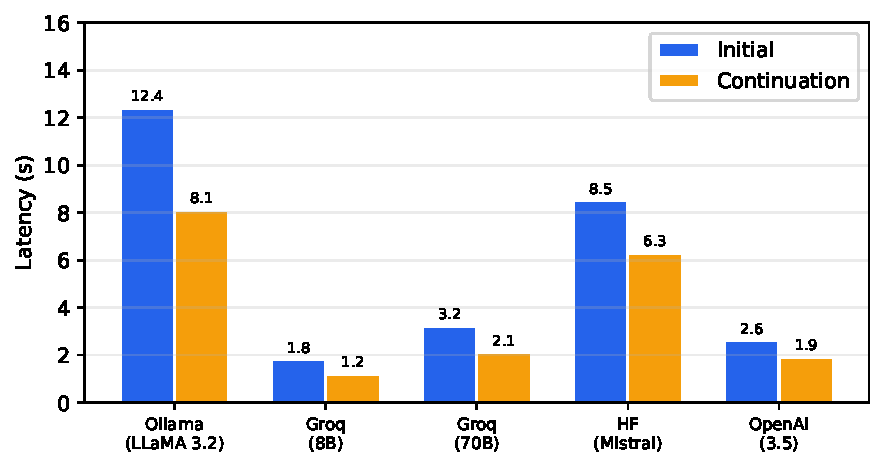
\includegraphics[width=0.85\textwidth]{images/f01_latency.pdf}
    \caption{Mean latency by LLM provider ($n=10$ calls per cell).}
    \label{fig:latency}
\end{figure}

Figure~\ref{fig:breakdown} breaks the total time of one interactive turn into its stages. At small question budgets the largest single cost is image synthesis (about 3.5\,s), but this runs in parallel with the LLM call and so adds little waiting time. At the Full budget of 17 questions, the time the user spends answering is the largest part.

\begin{figure}[H]
    \centering
    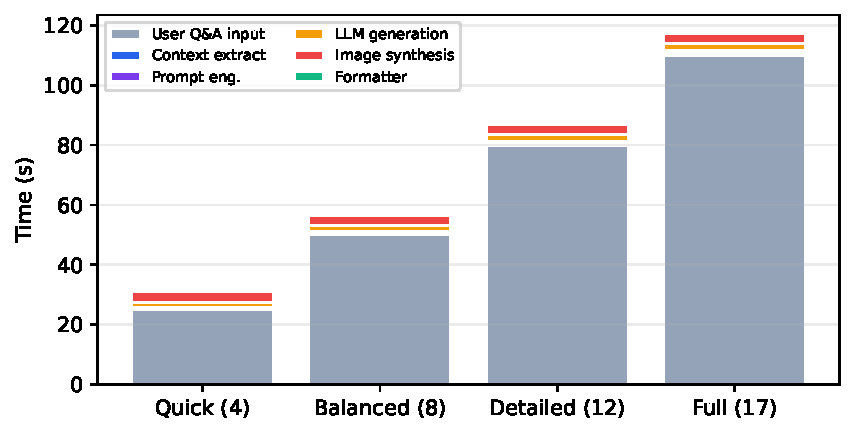
\includegraphics[width=0.85\textwidth]{images/f17_breakdown.pdf}
    \caption{Time of one interactive turn, divided by stage.}
    \label{fig:breakdown}
\end{figure}

\subsection{Narrative Quality}

Across all stories, the mean Likert scores were 4.05 for coherence, 4.12 for creativity, 4.35 for engagement and 3.75 for consistency. Figure~\ref{fig:quality} shows the scores by genre. Adventure received the highest engagement score (4.6). Mystery received the lowest consistency score (3.5), which is expected because a mystery depends on clues that must stay consistent across many segments. Figure~\ref{fig:tokens} shows the number of tokens per segment for each genre.

\begin{figure}[H]
    \centering
    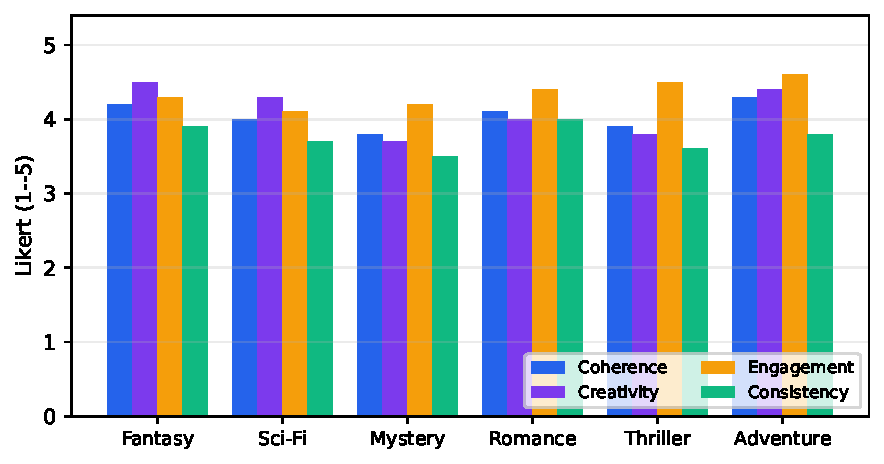
\includegraphics[width=0.85\textwidth]{images/f02_quality.pdf}
    \caption{Narrative quality by genre (Likert 1--5, $n=30$ stories).}
    \label{fig:quality}
\end{figure}

\begin{figure}[H]
    \centering
    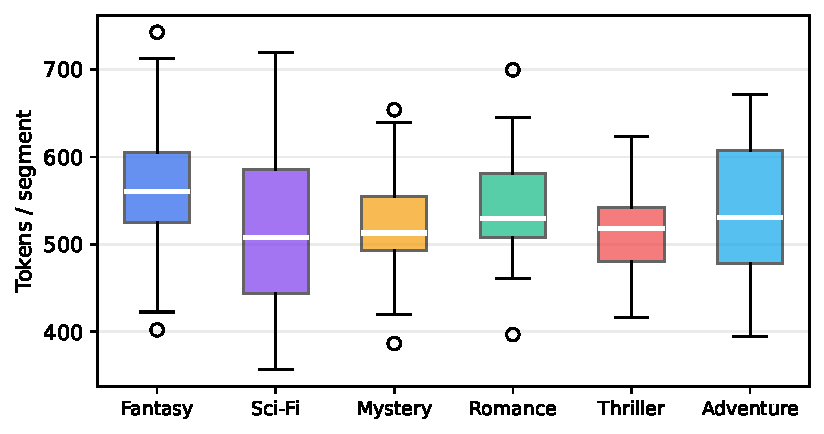
\includegraphics[width=0.85\textwidth]{images/f15_tokens.pdf}
    \caption{Tokens per segment by genre ($n=25$ segments each).}
    \label{fig:tokens}
\end{figure}

\subsection{User Satisfaction}

Figure~\ref{fig:satisfaction} shows satisfaction with seven features. The overall satisfaction was 4.3 out of 5. Custom answers (4.5) and image illustration (4.2) received the highest ratings, and genre alignment of the ambient music was rated 4.3. The lowest rating was for how meaningful the offered choices were (3.9). The choices are written by the language model, and free-tier models tend to suggest generic continuations.

\begin{figure}[H]
    \centering
    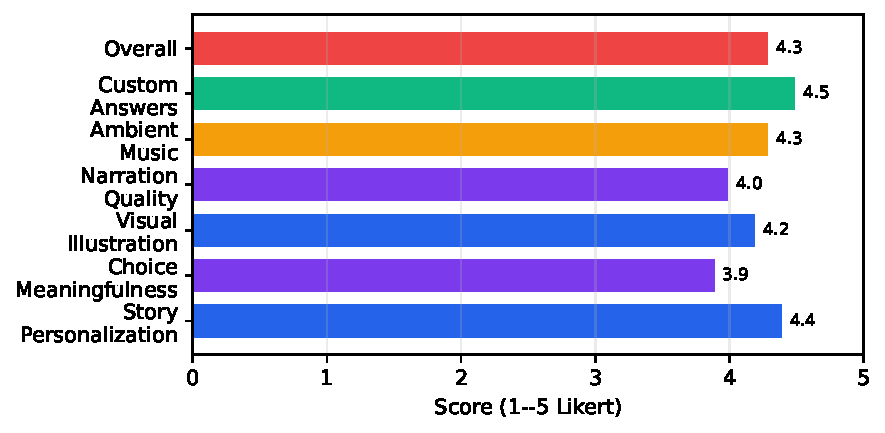
\includegraphics[width=0.85\textwidth]{images/f03_satisfaction.pdf}
    \caption{User satisfaction by feature (Likert 1--5, $n=15$ participants).}
    \label{fig:satisfaction}
\end{figure}

\subsection{Consistency-Checker Performance}

Figure~\ref{fig:consistency} gives the detection rate and false-positive rate of the consistency checker for each problem type. Character contradictions were detected best, with 87\% detection and 8\% false positives. Tone shifts were detected worst, with 68\% detection and 22\% false positives. A change of tone is spread across word choice and rhythm, and the keyword-based checker cannot capture it well.

\begin{figure}[H]
    \centering
    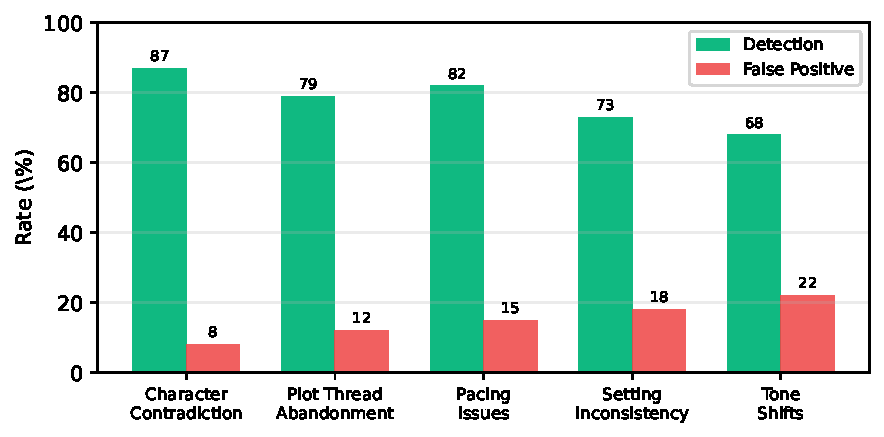
\includegraphics[width=0.85\textwidth]{images/f06_consistency.pdf}
    \caption{Consistency-checker detection and false-positive rates ($n=50$ segments).}
    \label{fig:consistency}
\end{figure}

\subsection{Image-Synthesis Throughput}

Figure~\ref{fig:imgthroughput} shows image latency against prompt length for serial requests, and the failure rate when five requests are sent in parallel without the queue. When requests were sent in parallel, the failure rate rose from about 40\% for 80-character prompts to about 98\% for 380-character prompts, with a sharp rise above about 230 characters. This is why the prompt is limited to 200 characters. With the serial queue and 1.2\,s spacing, failures fell from about 70\% to under 2\%, and the success rate after retries was above 95\%.

\begin{figure}[H]
    \centering
    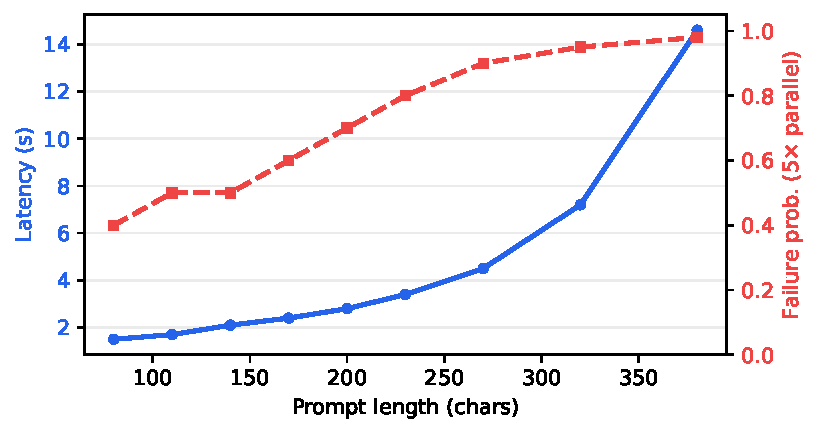
\includegraphics[width=0.85\textwidth]{images/f12_imgthroughput.pdf}
    \caption{Image latency against prompt length, and failure rate under parallel requests.}
    \label{fig:imgthroughput}
\end{figure}

\subsection{Character-Extraction Quality}

Figure~\ref{fig:char} compares a simple regular-expression extractor with the filtered version used in the system (extended stop-word list and a minimum of two mentions). Precision rose from 0.61 to 0.83, recall fell slightly from 0.84 to 0.78, and the $F_1$ score rose from 0.71 to 0.80. The false-positive rate fell from 0.39 to 0.17. The graph built from these names shows how often characters appear together, not what their relationship is, and the interface says so.

\begin{figure}[H]
    \centering
    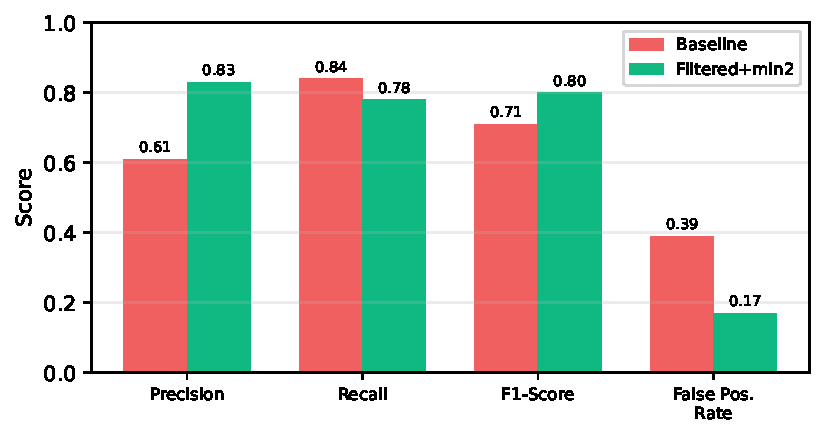
\includegraphics[width=0.85\textwidth]{images/f11_char.pdf}
    \caption{Character-extraction quality before and after filtering.}
    \label{fig:char}
\end{figure}

\subsection{Ambient-Music Frequency Profile}

Figure~\ref{fig:ambient} shows the relative energy in six frequency bands for each genre's music. Horror and thriller tracks have most of their energy in the sub-bass and bass bands, while comedy and adventure tracks have more energy in the middle and upper-middle bands. Participants rated the match between music and genre at 4.3 out of 5.

\begin{figure}[H]
    \centering
    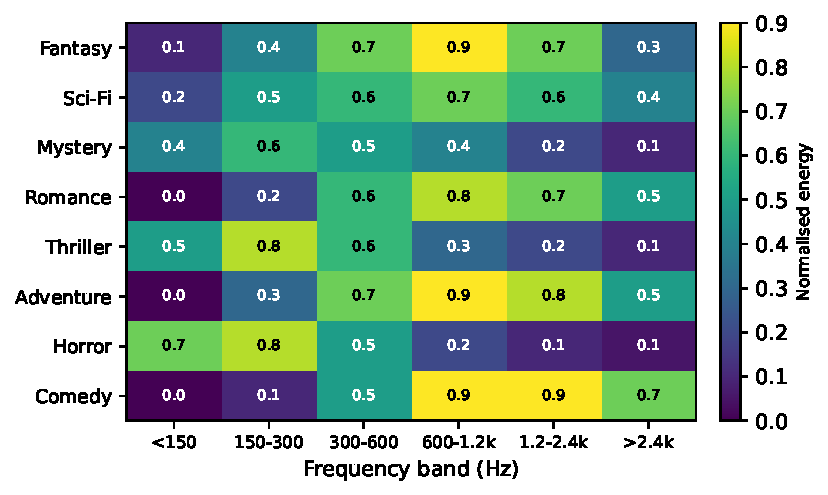
\includegraphics[width=0.85\textwidth]{images/f13_ambient.pdf}
    \caption{Energy by frequency band for each genre's ambient track.}
    \label{fig:ambient}
\end{figure}

\subsection{Question-Budget Ablation}

Table~\ref{tab:budget} gives the mean scores for each question budget. Personalisation rose steadily with the number of questions, from 3.2 at 4 questions to 4.6 at 17, a gain of about 1.4 points. Coherence rose more modestly, from 3.6 to 4.3 (0.7 points). Coherence and creativity reached their highest values at around 12 questions and changed little after that, while the time spent answering kept growing. A budget of 12 questions therefore gives the best balance and is the recommended default.

\begin{table}[H]
\centering
\caption{Mean Likert scores by question budget ($n=15$).}
\label{tab:budget}
\renewcommand{\arraystretch}{1.2}
\begin{tabular}{|l|c|c|c|c|}
\hline
\textbf{Budget} & \textbf{Coherence} & \textbf{Creativity} & \textbf{Personalisation} & \textbf{Time} \\
\hline
4 (Quick)     & 3.6 & 3.8 & 3.2 & 45\,s \\
8 (Balanced)  & 3.9 & 4.1 & 3.8 & 1.5\,min \\
12 (Detailed) & 4.2 & 4.2 & 4.3 & 2.5\,min \\
17 (Full)     & 4.3 & 4.1 & 4.6 & 3.5\,min \\
\hline
\end{tabular}
\end{table}

\subsection{Feature Adoption}

Figure~\ref{fig:adoption} shows the share of user-study sessions in which each feature was used at least once. Image generation, which is on by default, was used in 91\% of sessions. Ambient music and custom answers, which the user has to turn on, were used in 71\% and 62\% of sessions.

\begin{figure}[H]
    \centering
    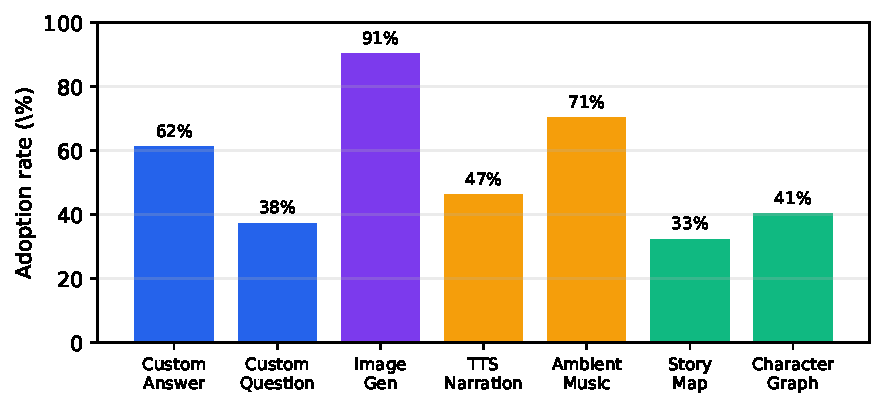
\includegraphics[width=0.85\textwidth]{images/f14_adoption.pdf}
    \caption{Share of user-study sessions in which each feature was used.}
    \label{fig:adoption}
\end{figure}

\subsection{Comparison with Existing Systems}

Figure~\ref{fig:radar} compares the proposed system with AI Dungeon, Dramatron and NovelAI on seven dimensions. The proposed system scores highest on deployment flexibility, cost, multimodal coverage and openness. AI Dungeon scores slightly higher on user control because it accepts free-form input, and Dramatron scores higher on raw coherence because of its hierarchical planner. No single existing system covers the same combination of strengths.

\begin{figure}[H]
    \centering
    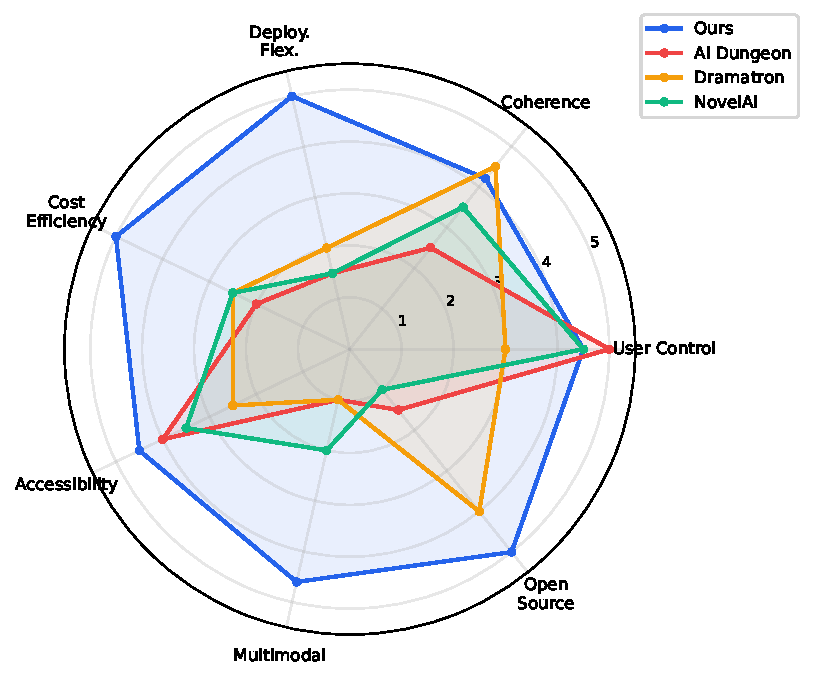
\includegraphics[width=0.85\textwidth]{images/f05_radar.pdf}
    \caption{Comparison with existing systems on seven dimensions.}
    \label{fig:radar}
\end{figure}

\subsection{Summary of Findings}

Table~\ref{tab:targetresults} compares the results with the targets set in Chapter~\ref{ch:intro}.

\begin{table}[H]
\centering
\caption{Results against the targets set at the start of the work.}
\label{tab:targetresults}
\renewcommand{\arraystretch}{1.2}
\small
\begin{tabular}{|l|c|c|c|}
\hline
\textbf{Metric} & \textbf{Target} & \textbf{Result} & \textbf{Met} \\
\hline
User satisfaction              & $>$ 4.0/5 & 4.3/5                & Yes \\
Response latency (cloud)       & $<$ 5\,s  & 1.8\,s (Groq)        & Yes \\
Image generation success       & $>$ 95\%  & $>$ 95\% after retry & Yes \\
Mean Likert (four dimensions)  & $>$ 3.8   & 4.07                 & Yes \\
Personalisation at 12 questions & --      & 4.3/5                & -- \\
Character-extraction $F_1$     & --        & 0.80                 & -- \\
\hline
\end{tabular}
\end{table}

The main findings are: (i) the system produces stories that users rate highly for engagement and creativity; (ii) the free Groq tier is fast enough for interactive use; (iii) the serial queue makes free image generation reliable; (iv) more questions give more personalised stories, with 12 questions as the best balance; and (v) consistency, especially of tone and of mystery plots, is the weakest area.

\section{Discussion}

\subsection{Introduction}

This section interprets the results, compares them with earlier work, and considers what they mean in practice and where the study is limited.

\subsection{Interpretation of Results}

The results support the central idea of this dissertation: a structured Q\&A protocol, combined with a provider-independent LLM backend and well-paced multimodal output, improves personalisation and engagement without harming coherence. The ablation shows the effect of the Q\&A step directly. Each additional group of questions raised personalisation, and coherence also improved, which suggests that the extra information helps the model write a more focused story rather than constraining it.

The features rated highest were custom answers and image illustration. Both are cheap to build; the first is a small interface addition and the second a free API call. Their high ratings show that giving users a voice and a visual result matters more to them than small changes in text quality. The weakest points, choice meaningfulness and tone consistency, depend mostly on the language model and on the keyword-based checker, not on the framework itself.

\subsection{Comparison with Previous Research}

Planning-based systems such as Dramatron~\citep{mirowski2023dramatron} and the approach of Farrell et al.~\citep{farrell2024narrative} achieve strong structure but do not involve the user during generation. The proposed system reaches comparable structure through the five-phase model while keeping the user involved at every turn. Free-form systems such as AI Dungeon~\citep{walton2019aidungeon} give more freedom but leave the user without guidance; studies of writing tools~\citep{liu2023endusers,yuan2022wordcraft} found that scaffolded interfaces help novice users, and the high engagement and custom-answer ratings in this study agree with that finding. Illustrated-story prototypes~\citep{schuhmann2024visualstory,bouhuis2024crossmodal} reported higher engagement when pictures match the text; this study observed the same effect in a deployed system and also solved the practical problem of rate limits, which those prototypes did not address.

\subsection{Implications of the Findings}

For educators, the system can produce personalised story-based material that follows a learner's interests. For game designers, the Q\&A pattern is a way to collect rich player preferences while keeping narrative control. For therapists, it offers a narrative tool that respects the user's choices. For content creators, it shows that personalised illustrated stories can be produced at almost no infrastructure cost. For researchers, the open-source code~\citep{jha2026repo} provides a baseline for further work, and the \texttt{custom\_elements} pattern can be reused in any LLM application that needs user-extensible personalisation.

\subsection{Limitations of the Study}

The study has several limitations:

\begin{itemize}
    \item Context extraction uses keywords and misses answers that are phrased differently; a fine-tuned DistilBERT~\citep{sanh2019distilbert} or zero-shot LLM classifier would improve recall.
    \item Sessions are held in memory, which limits scaling to several servers.
    \item The consistency checker is pattern based and has no semantic understanding; cross-segment natural-language inference~\citep{williams2018mnli} would be a natural upgrade.
    \item Image quality is limited by Pollinations.ai; a local SDXL~\citep{podell2024sdxl} or FLUX.1~\citep{bfl2024flux} model would give more consistent images but would require a GPU.
    \item Ambient music is streamed from an external CDN, which is a single point of dependency.
    \item The character graph shows co-appearance only, not the type of relationship.
    \item The user study had 15 participants aged 22--35, which is small and not diverse; a larger and broader group would strengthen the results.
\end{itemize}

\subsection{Recommendations for Future Research}

Future studies should use a larger and more varied group of participants, compare several language models under the same prompts, and add automatic measures of narrative quality~\citep{lin2024evalnarrate} alongside human ratings. Semantic methods for context extraction and consistency checking are the most promising way to raise the consistency score, which was the weakest result in this study. Detailed directions are given in Chapter~\ref{ch:conclusion}.

\chapter{Conclusion and Future Scope}
\label{ch:conclusion}

\section{Summary of the Study}

This dissertation set out to change how people take part in AI-generated stories, from passive readers to active co-authors. It presented the design, implementation and evaluation of a Q\&A based interactive storytelling system built on large language models. A protocol of 17 questions over four narrative dimensions (setting, character, theme and plot) collects the user's preferences, a seven-module backend turns them into a structured context and phase-specific prompts, and a provider-independent LLM layer generates the story. A five-phase model based on Freytag's pyramid keeps the plot moving from introduction to resolution, and a consistency checker watches for contradictions.

The text is supported by a scene illustration for each segment, generated through Pollinations.ai with a sentence-scoring prompt extractor and a serial request queue, by narration through the Web Speech API, and by ambient music chosen by genre. Readers can explore the story through a Story Map and a Character Relationship Graph. Users can write their own answers and add their own questions, which reach the model through the \texttt{custom\_elements} context channel.

\section{Main Findings}

\begin{itemize}
    \item Across 50 generated stories and 15 user-study participants, the system achieved mean Likert scores of 4.05 for coherence, 4.12 for creativity, 4.35 for engagement and 3.75 for consistency, with an overall satisfaction of 4.3 out of 5.
    \item Groq's free LLaMA-3.1-8B service produced the first segment in 1.8\,s on average, much faster than local Ollama (12.4\,s) and faster than paid OpenAI GPT-3.5-turbo (2.6\,s).
    \item Personalisation rose from 3.2 at 4 questions to 4.6 at 17 questions. A budget of 12 questions gave a personalisation score of 4.3 with under three minutes of answering, and is the recommended default.
    \item The serial request queue reduced image-generation failures under parallel load from about 70\% to under 2\%.
    \item Filtering with an extended stop-word list and a two-mention threshold raised the character-extraction $F_1$ score from 0.71 to 0.80 and more than halved the false-positive rate.
    \item Custom answers (4.5) and image illustration (4.2) were the most valued features, while the meaningfulness of suggested choices (3.9) and tone consistency were the weakest areas.
\end{itemize}

\section{Contributions to Knowledge}

\begin{enumerate}
    \item A Q\&A framework for interactive storytelling that personalises stories through a structured conversation over four narrative dimensions with selectable budgets.
    \item The \texttt{custom\_elements} context channel, a reusable pattern that lets end users add their own questions and have the answers reach the model's prompt without any change to code or schema.
    \item A sentence-scoring prompt extractor that removes dialogue and inner thoughts before story text is sent to a text-to-image model.
    \item A serial request queue that makes free, rate-limited image services reliable enough for interactive use.
    \item An openly labelled co-appearance character graph, as an example of honest reporting for visualisations whose basis is statistical rather than semantic.
\end{enumerate}

\section{Practical Implications}

The system shows that a complete multimodal storytelling application can be built from free components and run on a single laptop. Educators can use it to create personalised learning stories, game designers can adopt the Q\&A pattern to capture player preferences, therapists can explore it as a narrative tool, and content creators can prototype personalised illustrated stories at almost no cost. The open-source code~\citep{jha2026repo} gives other researchers a working baseline.

\section{Future Scope}

The work can be extended in several directions:

\begin{itemize}
    \item \textbf{Semantic context extraction} with DistilBERT~\citep{sanh2019distilbert} or zero-shot LLM classification in place of keyword dictionaries.
    \item \textbf{Semantic consistency checking} using natural-language inference between segments~\citep{williams2018mnli}.
    \item \textbf{Relationship extraction} for the character graph, so that it shows the kind of relationship and its sentiment, not only co-appearance.
    \item \textbf{Local image generation} with SDXL~\citep{podell2024sdxl} or FLUX.1~\citep{bfl2024flux} for offline use and consistent character appearance across images.
    \item \textbf{Neural narration} with models such as XTTS~\citep{casanova2024xtts}, giving each character its own voice.
    \item \textbf{Mood-based music} that changes with each segment instead of one track per genre.
    \item \textbf{Multi-user sessions} in which several people answer questions and take turns shaping the story.
    \item \textbf{Scalable deployment} with Docker containers and Redis-backed sessions.
    \item \textbf{Automatic evaluation} with measures such as BLEU, chrF, MAUVE and narrative-arc detection~\citep{lin2024evalnarrate}.
    \item \textbf{Genre-specific fine-tuning} with LoRA adapters trained on open story collections.
    \item \textbf{Multilingual support}, starting with Hindi and Marathi, to reach more users.
\end{itemize}

\section{Research Outcomes}

The work carried out in this dissertation has produced the following outcomes:

\begin{itemize}
    \item A working, open-source Q\&A based interactive storytelling application~\citep{jha2026repo}.
    \item A research paper, ``Q\&A-Driven Interactive Storytelling Using Large Language Models: A Multimodal Framework for Personalised Narrative Generation'', prepared from this work.
    \item User-study material, including the questionnaire, the ratings and the scripts used to produce the figures in this report.
\end{itemize}

\section{Final Thoughts}

Large language models have made high-quality text generation available to every developer, but turning text generation into a good storytelling experience is a design problem as much as a technical one. This dissertation argued that the key is a clear separation between what the system asks the user and what it does with the answers. By making the questions structured but open to extension, the language model replaceable, and the images, narration and music part of one coordinated experience, the system offers storytelling that is easy for first-time users and open to those who want to shape it further.


% Revert font size to original if needed for other parts
\fontsize{12}{14.4}\selectfont

% Bibliography
\bibliographystyle{abbrvnat}

\bibliography{references}
% \addcontentsline{toc}{chapter}{Bibliography}
%\printbibliography

\begin{appendices}

\chapter{Sample API Exchange}

The following request and response were captured during the user study. They show how a user-added question (\texttt{custom\_q\_1}) travels through the normal response path into the story prompt.

\begin{lstlisting}
POST /api/story/generate
{
  "session_id": "a1b2c3d4-...",
  "responses": {
    "setting_1":  "A magical fantasy realm",
    "char_1":     "Elena",
    "char_2":     "Brave and resourceful",
    "theme_1":    "Fantasy",
    "plot_1":     "Person vs. Supernatural",
    "custom_q_1": "Should the protagonist have an animal
                   companion? -> Yes, a silver fox"
  }
}

HTTP/1.1 200 OK
{
  "content":       "In the realm of Aethermoor...",
  "word_count":    387,
  "segment_count": 1,
  "phase":         "introduction",
  "choices": ["Explore further", "..."]
}
\end{lstlisting}

\chapter{System Summary and Reproducibility}

\begin{table}[H]
\centering
\caption{Summary of the final system.}
\renewcommand{\arraystretch}{1.2}
\begin{tabular}{|l|l|}
\hline
\textbf{Item} & \textbf{Value} \\
\hline
Backend modules          & 7, plus \texttt{main.py}, \texttt{config.py}, \texttt{run.py} \\
Database tables          & 5 \\
Questions                & 17 across 4 phases \\
LLM providers            & 4 (Ollama, Groq, Hugging Face, OpenAI) \\
Image generation         & Pollinations.ai \\
Narration                & W3C Web Speech Synthesis \\
Ambient music            & SoundHelix (8 genres) \\
Export formats           & TXT, Markdown, HTML \\
Story phases             & 5 (Freytag) \\
Visualisations           & Story Map, Character Graph (D3) \\
Stories evaluated        & 50 \\
User-study participants  & 15 \\
\hline
\end{tabular}
\end{table}

All experiments were run on macOS~14 with Python 3.11.5, \texttt{matplotlib} 3.9.4 and \texttt{numpy} 2.0.2. Image timings were measured over a 100\,Mbps residential connection; on slower connections the spacing of the serial queue should be increased. The source code, the user-study questionnaire and the figure-generation scripts are available at \url{https://github.com/DeepPatange/AI-Stroy-Generator}.

\end{appendices}

\end{document}
